\documentclass[12pt,a4paper]{report}

%% Verze pro jednostranný tisk:
% Okraje: levý 40mm, pravý 25mm, horní a dolní 25mm
% (ale pozor, LaTeX si sám přidává 1in)
\setlength\textwidth{145mm}
\setlength\textheight{247mm}
\setlength\oddsidemargin{15mm}
\setlength\evensidemargin{15mm}
\setlength\topmargin{0mm}
\setlength\headsep{0mm}
\setlength\headheight{0mm}

% \openright zařídí, aby následující text začínal na pravé straně knihy
\let\openright=\clearpage

%% Použité kódování znaků
\usepackage[utf8]{inputenc}

%% Ostatní balíčky
\usepackage{graphicx}
\usepackage{amsmath}
\usepackage{amssymb}
\usepackage{latexsym}
\usepackage{mathtools}
%\usepackage{amsfonts}
\usepackage[noend]{algpseudocode}
\usepackage{algorithm}
\usepackage{url}
\usepackage{afterpage}
\usepackage{natbib}
\usepackage{rotating}
\usepackage{multirow}
%\usepackage{multicol}
\usepackage{tocbibind}
\usepackage[usenames,dvipsnames]{color}
\usepackage{subfig}

%% Balíček hyperref, kterým jdou vyrábět klikací odkazy v PDF,
%% ale hlavně ho používáme k uložení metadat do PDF (včetně obsahu).
\usepackage[hidelinks]{hyperref}
\hypersetup{pdftitle=Measures of Machine Translation Quality}
\hypersetup{pdfauthor=Matouš Macháček}

% Tato makra přesvědčují mírně ošklivým trikem LaTeX, aby hlavičky kapitol
% sázel příčetněji a nevynechával nad nimi spoustu místa. Směle ignorujte.
%\makeatletter
%\def\@makechapterhead#1{
%  {\parindent \z@ \raggedright \normalfont
%   \Huge\bfseries \thechapter. #1
%   \par\nobreak
%   \vskip 20\p@
%}}
%\def\@makeschapterhead#1{
%  {\parindent \z@ \raggedright \normalfont
%   \Huge\bfseries #1
%   \par\nobreak
%   \vskip 20\p@
%}}
%\makeatother

\def\parcite#1{\citep{#1}}
\def\perscite#1{\cite{#1}}

% Deklarace stylů fontů pro různé druhy termínů
\newcommand{\metric}[1]{\textsc{#1}}
\newcommand{\system}[1]{\textsc{#1}}
\newcommand{\pojem}[1]{\texttt{#1}}
\newcommand{\metoda}[1]{\textbf{#1}}
\newcommand{\script}[1]{\texttt{#1}}
\newcommand{\XXX}[1]{\textcolor{Red}{XXX #1}}
%\newcommand{\XXX}[1]{}
\newcommand{\best}[1]{\textbf{#1}}
\def\oosmark#1{\llap{$\wr$\,}#1}  % out-of-sequence mark
\newcommand*\Let[2]{\State #1 $\gets$ #2}
\newcommand{\hit}[1]{\textcolor{OliveGreen}{\textbf{#1}}}
\newcommand{\miss}[1]{\textcolor{Red}{\textbf{#1}}}


\begin{document}

% Trochu volnější nastavení dělení slov, než je default.
\lefthyphenmin=2
\righthyphenmin=2

%%% Titulní strana práce

\pagestyle{empty}
\begin{center}

\large

Charles University in Prague

\medskip

Faculty of Mathematics and Physics

\vfill

{\bf\Large MASTER THESIS}

\vfill

\centerline{\mbox{
\includegraphics[width=60mm]{img/logo}}}

\vfill
\vspace{5mm}

{\LARGE Matouš Macháček}

\vspace{15mm}

% Název práce přesně podle zadání
{\LARGE\bfseries Measures of \\ Machine Translation Quality}

\vfill

% Název katedry nebo ústavu, kde byla práce oficiálně zadána
% (dle Organizační struktury MFF UK)
Institute of Formal and Applied Linguistics

\vfill

\begin{tabular}{rl}

Supervisor of the master thesis: & RNDr. Ondřej Bojar, Ph.D. \\
\noalign{\vspace{2mm}}
Study programme: & Computer Science \\
\noalign{\vspace{2mm}}
Specialization: & Mathematical Linguistics \\
\end{tabular}

\vfill

% Zde doplňte rok
Prague 2014

\end{center}

\newpage

%%% Následuje vevázaný list -- kopie podepsaného "Zadání diplomové práce".
%%% Toto zadání NENÍ součástí elektronické verze práce, nescanovat.

%%% Na tomto místě mohou být napsána případná poděkování (vedoucímu práce,
%%% konzultantovi, tomu, kdo zapůjčil software, literaturu apod.)

\openright

\noindent
\XXX{Dedication.}

\newpage

%%% Strana s čestným prohlášením k diplomové práci

\vglue 0pt plus 1fill

\noindent
I declare that I carried out this master thesis independently, and only with the cited
sources, literature and other professional sources.

\medskip\noindent
I understand that my work relates to the rights and obligations under the Act No.
121/2000 Coll., the Copyright Act, as amended, in particular the fact that the Charles
University in Prague has the right to conclude a license agreement on the use of this
work as a school work pursuant to Section 60 paragraph 1 of the Copyright Act.

\vspace{10mm}

\hbox{\hbox to 0.5\hsize{%
In Prague, 31th of July 2014 
\hss}\hbox to 0.5\hsize{%
%signature of the author
\hss}}

\vspace{20mm}
\newpage

%%% Povinná informační strana diplomové práce

\vbox to 0.5\vsize{
\setlength\parindent{0mm}
\setlength\parskip{5mm}

Název práce:
Měření kvality strojového překladu

Autor:
Matouš Macháček

Ústav:
Ústav formální a aplikované lingvistiky

Vedoucí diplomové práce:
RNDr. Ondřej Bojar, Ph.D., UFAL

Abstrakt:
\XXX{Napsat Abstrakt v cestine}

Klíčová slova:
strojový překlad, vyhodnocování kvality, automatické metriky, anotace

\vss}\nobreak\vbox to 0.49\vsize{
\setlength\parindent{0mm}
\setlength\parskip{5mm}

Title:
Measures of Machine Translation Quality

Author:
Matouš Macháček

Department:
Institute of Formal and Applied Linguistics

Supervisor:
RNDr. Ondřej Bojar, Ph.D., UFAL

Abstract:
\XXX{Napsat Abstrakt v anglictine}

Keywords:
machine translation, quality measurement, automatic metrics, annotation

\vss}

\newpage

%%% Strana s automaticky generovaným obsahem diplomové práce. U matematických
%%% prací je přípustné, aby seznam tabulek a zkratek, existují-li, byl umístěn
%%% na začátku práce, místo na jejím konci.

\openright
\pagestyle{plain}
\setcounter{page}{1}
\tableofcontents

%%% Jednotlivé kapitoly práce jsou pro přehlednost uloženy v samostatných souborech
\chapter{Introduction}

The field of machine translation (MT) experienced a very fast development over
the past twenty years. It was primarily caused by the growing power of
computers which allowed researchers to start using statistical methods which
require a lot of computer resources to both learn statistics from data and then
to use them in translation.

In the globalized world we live in, there is a need for translating from one
human language to another. The translation itself is often not easy even for
people who have to be trained for that and therefore well paid. There is
therefore a very high demand for cheap and high-quality machine translation. A
lot of researchers and companies try to satisfy this demand and constantly
improve their translations system. The first presumption for improving your
system is that you know how to measure the improvement.

There are a lot of situations in which you need to evaluate machine
translation. If you are a customer who would like to buy a machine translation
system you want to buy the system which will best suit you. There are many
criteria of MT systems (speed, price, memory consumption, scalability etc.) but
the most important criterion is usually the machine translation quality.
Therefore, you would like to evaluate this quality on a sample of documents you
are going to translate.

If you are a developer of a machine translation system you need to evaluate
your system during various phases of the development process. Let us go through
the phases which need an evaluation in reversed order. From time to time, you
have a ready-to-use system and you would like to have a comparison to systems
of your competitors or another researchers. You can evaluate your system
yourself in a way that the obtained score is comparable to other scores, or you
can participate in a shared evaluation campaign, for instance NIST
OpenMT\footnote{\url{http://www.nist.gov/itl/iad/mig/openmt12.cfm}} or at
Workshop on Statistical Machine
Translation\footnote{\url{http://www.statmt.org/wmt14/translation-task.html}}
(WMT) organized by \perscite{wmt14-overview-paper}.  During the day-to-day
development process of your system, you try various configuration, new
components and features. You have to evaluate your system with every change to
know how much the change improved (or sometimes worsen) the translation
quality. Recently, new automatic methods which tune parameters of your system
to directly optimize an evaluation measure emerged.

Unlike other applications of natural language processing, for instance speech
recognition, the evaluation in machine translation is not easy at all. The main
reason for that is that when translating an average sentence there is no single
correct solution, in fact there are hundreds of thousands correct translations
\parcite{bojar2013scratching}.

There are two fundamental approaches in the machine translation evaluation: a
manual evaluation and an automatic evaluation.  In the manual evaluation, human
judges assess the quality of each sentence manually. The most widely used
methodology in the past was to assign values from two five point scales
representing fluency and adequacy. However, it was shown that a) people had
difficulties with separating these two aspects of translation and b) there was
a very small inter-annotator agreement, since each annotator had different
expectation of a good translation. In later evaluation campaigns started by
\perscite{wmt-overview-2007}, annotators ranked translations relatively 
to each other.

In the automatic evaluation, an output of a machine translation system is
compared to a reference translation. However, Unlike other machine learning
problems, you cannot simply compute the proportion of translated sentences
which match the reference translation. If a translated sentence is not
identical to its reference counterpart it does not have to be a bad translation
because there is the very large number of correct translations. Automatic
metrics\footnote{Automatic metrics for machine translation evaluation are not
actually metrics according to the mathematical definition. For example, the
triangle inequality usually does not hold and some metrics are not even
symmetric. However, we are going to use this traditional term in this thesis.}
are used to measure the similarity between the candidate and reference
translations. The more similar they are, the better the translation is
considered.

As you can see, the evaluation of machine translation is very important and at
the same time, very difficult. We explore both manual and automatic evaluation
in this thesis.

\section{Motivation and Goals}

Manual evaluation is of course considered as the only source of truth to which
metrics try to approximate. However, it suffers from many disadvantages. Since
it includes manual labour, it is very costly and slow. Moreover, manual
evaluation is not reproducible; human judges have different criteria for
comparing candidates and even an individual judge is not consistent with
himself in time. Human evaluation is therefore most often used in shared
evaluation campaigns and rarely used when you want to evaluate a new component
of your system. It is definitely not feasible to directly use human evaluation
in an automatic method for tuning your model's parameters because these methods
require to evaluate millions of sentences.

Automatic metrics, on the other hand, are fast, reproducible and cost almost
nothing. However, they are only proxies to human evaluation and their
correlation to human judgments varies a lot. The first goal of this thesis is
therefore to conduct a large-scale comparison of available automatic metrics in
the terms of correlation with human judgments. For this purpose, we have
organized Metrics Shared Task within Workshop on Statistical Machine
Translation in two consecutive years 2013 \parcite{machacek:2013} and 2014
\parcite{machacek:2014}. We also compare the metrics in other more subjective
criteria. 

It would be very useful if we have an evaluation method which would take
advantages from both manual and automatic evaluations. Recently, there actually
emerged such methods on the boundary of manual and automatic evaluation. These
methods usually require a large manual annotation effort at the beginning to
create a database and then they use the collected database in an automatic way
during evaluation.  The second goal of this thesis is to propose a method which
could be used to manually evaluate a set of systems and the database collected
during this manual evaluation could be later reused to automatically evaluate
new, unseen systems and to tune a system. This goal includes, besides proposing
the method, also developing an annotation application, conducting a real
evaluation experiment and experiment with reusing the collected database. 

\section{Outline}

The outline of the thesis is following: In Chapter \ref{chapter:segranks} we
propose the manual evaluation method and report the annotation experiment. We
explore the possibility of reusing the collected database to evaluate new
systems and to tune a system in Chapter \ref{chapter:experiments}. The Automatic
metrics are are described, compared and evaluated in the terms of correlation
with human judgments in Chapter \ref{metrics}. Related work is summarized in
Chapter \ref{chapter:related}. You can find a documentation of the annotation
application and the tools for metrics evaluation in Chapter
\ref{chapter:implementation}. We conclude our work in Chapter
\ref{chapter:conclusion}.


\XXX{Kde citovat \parcite{bojar2012cestina}}



\begin{comment}
Machine Translation quality can be measured in two different ways: using human
evaluation or automatic metrics.  Altough human evaluation is considered more
accurate than automatic evaluation, it suffers some disadvantages.  It is slow
and expensive and therefore cannot be used in tuning parameters of statistical
models.

The aim of this thesis is to develop a new semi-automatic evaluation measure,
which would have advantages of both human evaluation and automatic evaluation.
The idea is to evaluate small sentence segments by human and create a database
of such annotation which could be used later to automatically evaluate new
unseen sentences.  This new measure should evaluate MT outputs more similarly
to how human do and still be cheap and fast after the initial database of
annotations is created once. It could be therefore used in tuning parameters of
MT systems.

The important part of the thesis is to design and develop a new annotation
environment which will be used to collect the annotations. This will be then used
to annotate wmt14 test data. The new measure will be analysed and compared to
current manual and automatic evaluation measures. 
\end{comment}






\chapter{Related Work}
\label{chapter:related}

\XXX{Tady bude reserse metod pro evaluaci MT. Popsat pouzivane zpusoby automaticke, rucni a poloautomaticke evaluace }


\XXX{Citovat MERT: Feasibility of Human in the loop}
\XXX{Citovat a popsat Scratching the surface of possible translations}
\XXX{Citovat An Evaluation Tool for Machine Translation: Fast Evaluation for MT Research}


\chapter{Proposed Semi-Automatic Evaluation Method}

The method we propose consists of two parts. The first part is a way how humans
judge outputs of judged systems. The second part is how to interpret collected
judgments to compute overall scores and rank the systems. We discuss these two
parts in following two sections. \XXX{V tomto odstavci (a asi i v dalsich odstavcich
neni dostatecne zdurazneno, proc je to semi-automaticka metoda, mozna opustit
oznaceni semi-automaticka a pouzit misto toho neco jako Manual Evaluation Method
with posibility to reuse collected judgementes for new systems)}

In the WMT official human evaluation humans judge whole sentences. They get
five candidate translations of a given source sentence and their task is to
rank these candidates relatively (ties are allowed). One of disadvantages of
this method is that sentences are quite long and therefore quite hard to
remember for judge to compare them. Also when comparing longer sentences there
are much more aspects in which one sentence can be better or worse than second
sentence and therefore it is more difficult for judges to choose the better
candidate. 

%\begin{algorithm}[H]
%    \KwData{Tree, MaxSegmentLength}
%    \KwResult{List of extracted segments}
%    \If{Tree covers more than MaxSegmentLength}{
%      yield all leaves \;
%    }
%    \caption{Segment extraction from parsed tree}
%    \label{segment:extraction}
%\end{algorithm}

To avoid these disadvantages we propose the following method. Instead of
judging whole sentences we extract shorter segments from candidates and give
them to judges to rank them. In order to extract meaningful segments with the
same meaning from all candidates we do the following procedure: First we parse
the source sentence and then we go recursively down the parsed tree and find
nodes which covers source segments with given maximum length (which is a
parameter of this method). This is exactly described in algorithm
\ref{segment:extraction}. Finally we project these extracted source segments to
their counterpart segments in all candidate sentences using an automatic
alignment.  You can find the whole process ilustrated in figure \XXX{nakreslit
obrazek}.  This extraction method is inspired by \XXX{citovat ten clanek a
stary WMT clanek}.

In \XXX{citovat WMT}, these extracted segments are only highlighted and shown
to judges together with the rest of the sentence. Judges are asked to rank the
segments in the context of whole sentences. \XXX{Zkontrolovat presne instrukce
z WMT}

We use different approach here which is more similar to that used in
\XXX{citovat ten clanek}. We show the extracted segments without any context
and ask judges to rank them. The only additional information provided to
annotators is the whole source sentence with the source segment highlighted.
Judges are told that they can imagine the rest of the sentence in which the
ranked segment fits best. They are instructed to penalize only those segments
for which they cannot imagine any appropriate rest of the sentence.

While we are aware that this approach has some disadvantages (which we
summarize bellow) there is one significant advantage: it is much more likely
that two systems produce the same translation of a short segment then they
would produce the same translation of a whole sentence. Because we do not show
the sentence context to annotators we can merge the equal segment candidates
into one, so the annotators have less candidate segments to rank. This also
allows us to reuse already collected human judgements later to evaluate a new
system which was not in the set of annotated systems (we present this
experiment in the section \ref{evaluating-new-systems}) or to tune parameters
of a system (we present this experiment in the section \ref{tuning-systems}).

\section{Data and Segment Preparation}

We have conducted an annotation experiment using the proposed method. In this
section we describe what data we have used and how we prepare them for the
annotation experiment.

We used English to Czech part of the WMT14 \parcite{wmt14-overview-paper} test
set. We choose this data set to be able to compare experiments' results with
the official WMT14 human evaluation. 

The testset consists of 3003 sentences (68866 tokens). It contains both source
sentences and reference translations. Roughly a half of the sentences was
originally in Czech and was translated by human translators into English. The
second half of the sentences was translated in opposite direction. Besides the
source and reference translations, we also used candidate translations of 10
systems which participated in the WMT14 translation task. All systems are
listed in the table \ref{translation-task-participants}


\begin{table}[h]
  \small
  \begin{center}
    \begin{tabular}{|l|l|l|}
      \hline
      \textbf{ID} & \textbf{Type} & \textbf{Team} \\
      \hline
      \system{cu-depfix} & statistical & \multirow{4}{*}{Charles University, Prague \XXX{(Tamchyna et al., 2014)}}  \\
      \system{cu-bojar} & statistical &  \\
      \system{cu-funky} & statistical &  \\
      \system{cu-tecto} & statistical &  \\
      \hline
      \system{uedin-phrase} & statistical &  \multirow{2}{*}{University of Edinburgh \XXX{(Durrani er al., 2014b)}} \\
      \system{uedin-uncnstr} &  statistical &  \\
      \hline
      \system{commercial-1} & rule-based & \multirow{2}{*}{Commercial machine translation systems} \\
      \system{commercial-2} & rule-based & \\
      \hline
      \system{online-a} & statistical & \multirow{2}{*}{Online statistical machine translation systems} \\
      \system{online-b} & statistical & \\
      \hline
    \end{tabular}
  \end{center}
  \caption{Systems participating WMT14 translation task in direction English-Czech \XXX{Zkontrolovat typy nekterych systemu}}
  \label{translation-task-participants}
\end{table}

Source sentences and all candidate translations were tokenized using the script
\script{tokenizer.perl}. Unicode punctuation characters were normalized using
the script \script{replace-unicode-punctuation.perl}. (Both scripts are included
in the Moses toolkit).

The source sentences were parsed using the Stanford lexicalized parser
\XXX{citace}. We used \pojem{englishFactored} model which is distributed with
the parser. (More models were examined and this model gave subjectively the
best segments). \XXX{Tady popsat detailneji, ktere modely jsem zkusil a ze 
to nebylo zase tak subjektivni}

We computed an alignments between the source sentecnes and the candidate
translations using Giza++ \XXX{citace}. Since the alignment algorithm is
unsupervised and the amount of all candidate translations is relatively small
($10 \times 3003$), we introduced more data by concatenating all candidate
translations with Europarl parallel corpus (646 605 sentences, \XXX{citovat})
and with \XXX{Jaky je to korpus?} (197 053 sentences, \XXX{citovat}).  The
concatenated parallel corpus was lowercased before alignment computation. 

We extracted short segments from the parsed source trees using the algorithm
\ref{segment:extraction}. The constant \pojem{min-segment-length} was set to
the value 3 to filter out very short segments which are hard to judge without
context. This also helped to reduce the number of extracted segments to be
annotated. The constant \pojem{max-segment-length} was set to the value 6 so
the extracted segments were not too long to judge and in the same time it was
more likely that two candidate translations of a segment were equal and
therefore there would be less items to rank (our aim was to make annotations as
easy and fast as possible). We have experimented with various settings of these
two constants and the final settings seemed to generate reasonable number of
meaningful segments.

\XXX{Nekde zduraznit, ze to jsou vlastne konstituenty, ale asi ne tady, nekde drive}

From 3003 source sentences, we have extracted 8485 segments of length 3 to 6
tokens. That is \XXX{priblizne} 2.83 segments on a sentence on average. By
projecting the source segments to the candidate sentences using the computed
alignments, we got $10 \times 8485 = 84850$ candidate segments. However, after
the merging of equal segments only 50011 candidate segments left. This is 58.9
\% of the original candidate segments, or in other words, after the merging we
got 5.89 (instead of original 10) candidate segments to be ranked for each
source segment on average. Theese prepared candidate segments were inserted
into the database to be ranked by annotators.

\section{Segments Ranking}

We have developed a new annotation application for this annotation
project.\footnote{It would be probably possible to customize and use an
    existing annotation application, for example Appraise\XXX{citovat}.
    However, since the ranking the short segments is quite specific it would
require a lot of customization. We therefore decided to develop our own
light-weight web application which would suit our needs perfectly and allow us
to optimize efficiency of the annotation.} For implementation details of this
application, please see the chapter \ref{implementation}. You can find an
example screen shot of this application in figure \ref{segranks-screenshot}.
Our goal was to make the annotation as efficient and user friendly as possible.
Annotators ranks all the source segments of a sentence at one screen (so that
they have to read the source sentence and reference translation only once). For
each annotated segment they see the source sentence repeated with the annotated
segment highlighted. Annotators rank the segment candidates by drag-and-droping
them to appropriate rank positions. After all candidates of all source segments
of a sentence are ranked annotators are allowed to submit the results to the
server.

The web interface is responsive, so it works correctly on mobile devices.
(Although ranking segments on a mobile phone is not very practical). The
drag-and-drop works also on touch screens.

\begin{figure}
    \begin{center}
        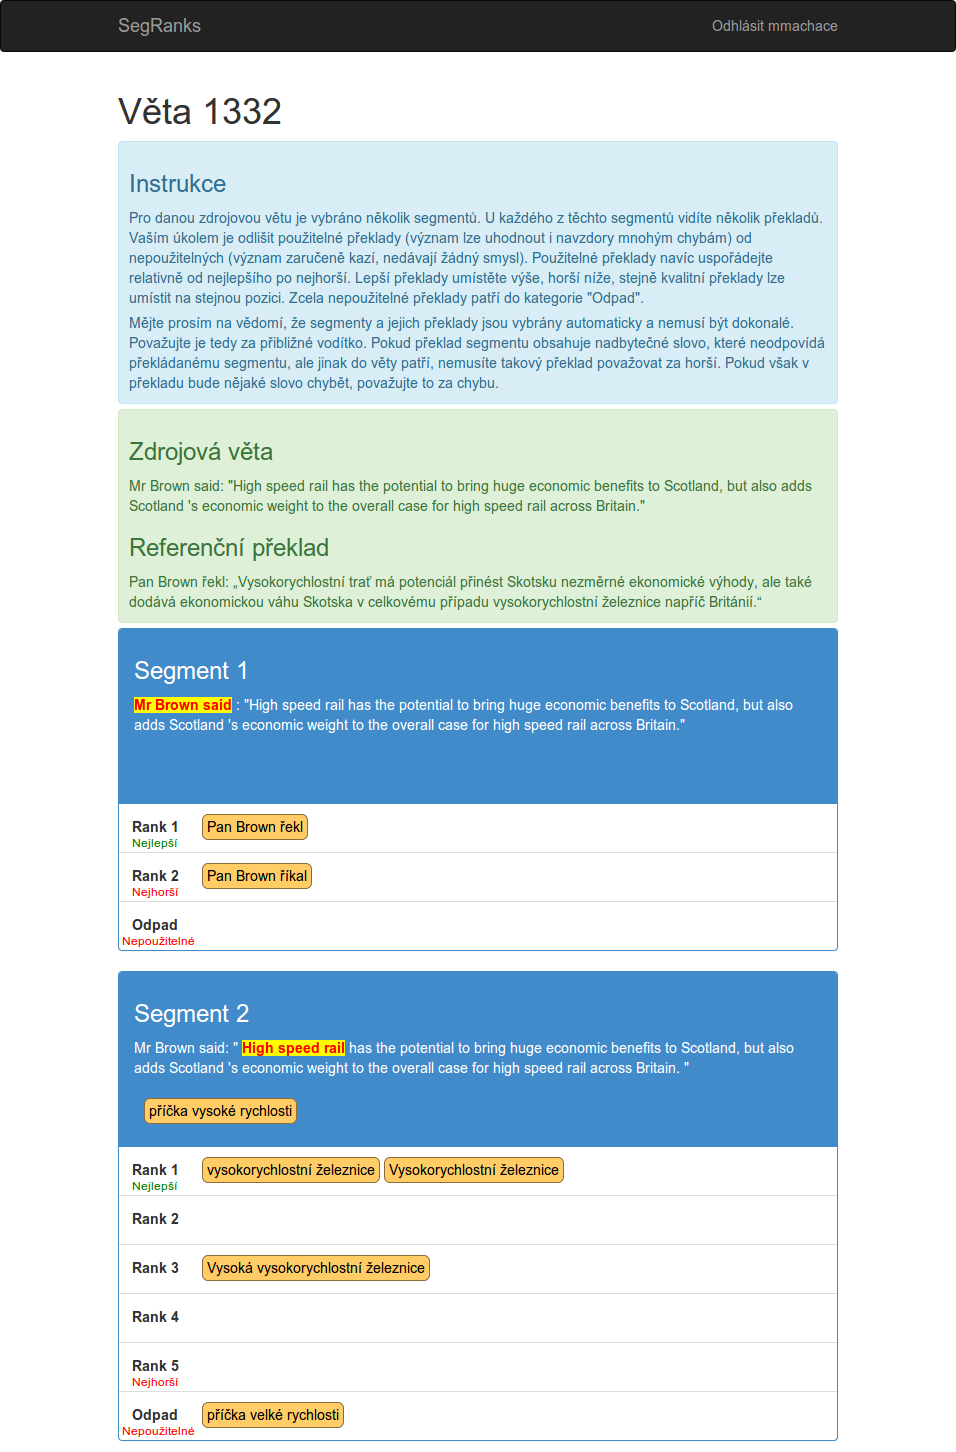
\includegraphics[width=\textwidth]{img/segranks-screenshot2.png}
    \end{center}
    \caption{A screenshot of an annotation application. Annotators rank the
    candidate segments by draging and dropping them into the ranks.
Annotators see all annotated segments of a sentence on single screen}
    \label{segranks-screenshot}
\end{figure}

\begin{quote}
A number of segments are extracted from the annotated sentence. You are shown a
few candidate translations for each of these segments. Your task is to
distinguish \XXX{vhodnejsi} the acceptable\XXX{vhodnejsi} candidate
translations (the meaning of the segment can be guessed despite a few or more
errors) from the unacceptable ones (the meaning is definitely not possible to
guess from the candidate segment). Also please rank the acceptable candidate
translations relatively from the best ones to the worst ones.  Please, place
better candidate translations higher, the worser ones lower. You can place
candidates of the same quality on the same rank. Please place the unacceptable
candidates to the position ``Garbage''

Please note that source segments and their candidate translations are chosen
automatically and does not have to be perfect. Consider them as only
\XXX{priblizne voditko}. If a candidate segment contains an extra word, which
does not correspond to the source segment but otherwise could be in the
translated sentence you do not have to consider such candidate as worser. If
something is missing in the candidate translation you should consider that as
an error.
\end{quote}

\XXX{zduraznit jednoduchost,
anotatori,  prubeh anotace, statistiky analyza
ziskane databaze, mezianotatorske shody, cena, platby}

\XXX{Je vubec slovo segment vhodne??? Span?? Constituent??}


\section{Experiments}

\subsection{Evaluating Annotated Systems}
\XXX{Zde uvedu vzorecek (mozna vice variant) pro vypocet skore systemu, ktere
byly anotovane. Vypocet skore, vypocet korelace s oficialnimi WMT14 vysledky.
Porovnani obou metod z hlediska mnozstvi lidske prace.}

\subsection{Evaluating New Systems}
\label{evaluating-new-systems}

\XXX{Zde zkusim pouzit vytvorenou databazi pro vyhodnoceni noveho systemu}

\XXX{provest experimenty podobne tem z clanku An Evaluation Tool for Machine
Translation: Fast Evaluation for MT Research}

\subsection{Tuning Systems}
\label{tuning-systems}

\XXX{Zde zkusim pouzit vytvorenou databazi pro MT tuning}

\section{Comparison to Other Manual Methods}

\chapter{Using Short Segments in MT Development}

In this chapter, we describe several experiments with the collected database of
annotations. 

\section{Overall Ranking of Annotated Systems}
\label{evaluating-annotated-systems}

In the first experiment, we would like to show that the proposed method can be
used to produce overall ranking of the annotated systems which will be very
similar to the official human evaluation in WMT with much less human effort
\XXX{dolozit, pokud je to vubec pravda a pokud to vubec pujde}.

The obtained database contains a list of annotations for each extracted source
segment from each source sentence. The list can be empty (not all of the
sentences were annotated), it can contain more than one annotation (some
segments were annotated twice by an annotator, some segments were annotated by
multiple annotators), but most of the time it contains only one annotation.

An annotation is a mapping from the set of candidate segments to the set of
ranks ${1 \ldots N+1}$, where $N$ is the count of unique candidate segments.
(To discriminate the relative quality of all segments, annotators had available
$N$ ranks which could be all occupied when there were no ties. The rank $N+1$
represents the ``garbage'' category from the annotation application. However in
all of our experiments reported in this thesis we consider this category simply as one
more, the worst, rank). A lower rank of a segment means that the candidate
segment was ranked better. This is an example \metoda{segment annotation} of a
source segment ``the huge volume'':

\begin{verbatim}
    {
      'velkému objemu' : 1,
      'obrovské hlasitosti' : 5,
      'obrovský objem' : 2,
      'obrovské množství' : 2,
    }
\end{verbatim}

We expanded these segment annotations with the information about the systems
which produced the segments. The ranks in the annotations are now indexed by
the system names.  If more systems translated a source segment as the same
candidate segment, the candidate segment's rank is copied to all the systems.
This is the time when we take advantage of ranking short segments which are
often translated identically.  The following is the \metoda{system annotation}
after expansion of the above \metoda{segment annotation}:

\begin{verbatim}
    {
      'uedin-unconstrained' : 2,
      'commercial1' : 5,
      'commercial2' : 2,
      'CU-TectoMT' : 1,
      'onlineB' : 2,
      'onlineA': 2,
      'cu-funky' : 2,
      'cu-bojar' : 2,
      'uedin-wmt14': 2,
      'cu-depfix': 2
    }
\end{verbatim}

These rankings are now very similar to those obtained in the official WMT human
evaluation. These annotations are mostly interpreted as pairwise systems'
comparisons (for each combination of size 2 of all systems we have a pairwise
comparison), where the absolute values of the ranks and their absolute
differences between them are not considered. From above \metoda{system
annotation}, the following \metoda{pairwise comparisons} are be extracted (only
a few extracted pairwise comparisons are listed here for the sake of brevity,
generally $N \times (N-1) / 2$ pairwise comparisons are extracted, where $N$ is
number of all systems):

\begin{verbatim}
    [
      'uedin-unconstrained' < 'commercial1',
      'uedin-unconstrained' = 'commercial2',
      'uedin-unconstrained' > 'CU-TectoMT',
      ...
      'commercial1' > 'commercial2',
      'commercial1' > 'CU-TectoMT',
      ...
    ]
\end{verbatim}

The interpretation of these pairwise comparisons has changed several times
during the WMT workshops. Here, we use \metoda{Ratio of wins (ignoring ties)}
method, which was introduced by \perscite{bojar:grain:of:salt} and used in
WMT12 workshop \parcite{callisonburch:wmt12}. This method is based on a method
used in several WMT workshops before WMT12 and it is quite easy to compute and
interpret results.

For a given set $C$ of segment-level extracted pairwise comparisons
$(s_1,s_2,c)$, where 

\begin{equation*}
c = \begin{cases}
  win  & \text{if $rank(s_1) < rank(s_2)$} \\
  loss & \text{if $rank(s_1) > rank(s_2)$} \\
  tie  & \text{if $rank(s_1) = rank(s_2)$} \\
    \end{cases}
\end{equation*}

\noindent we define for each system $s$ the total number of wins, losses and ties:

\begin{equation*}
\begin{array}{rcl} 
  win(s)  & := & |\{(s,\bar{s},c) \in C; c = win\}| + |\{(\bar{s},s,c) \in C; c = loss\}| \\
  loss(s) & := & |\{(s,\bar{s},c) \in C; c = loss\}| + |\{(\bar{s},s,c) \in C; c = win\}| \\
  ties(s) & := & |\{(s,\bar{s},c) \in C; c = tie\}| + |\{(\bar{s},s,c) \in C; c = tie\}| \\
\end{array}
\end{equation*}

Then the \metoda{Ratio of wins (ignoring ties)} for a given system $s$ is
computed using the following formula:

\begin{equation*}
  E_{win}(s) = \frac{win(s)}{win(s) + loss(s)} 
\end{equation*}

\begin{table}
  \begin{center}
    \subfloat[Short segments judgements]{
      %\begin{center}
        \begin{tabular}{|l|c|}
          \hline
          \textbf{System} & \textbf{Score} \\
          \hline
           cu-depfix           &  0.5777 \\
           onlineB             &  0.5642 \\
           uedin-unconstrained &  0.5626 \\
           cu-bojar            &  0.5606 \\
           cu-funky            &  0.5566 \\
           uedin-wmt14         &  0.5498 \\
           onlineA             &  0.5007 \\
           CU-TectoMT          &  0.4485 \\
           commercial1         &  0.3992 \\
           commercial2         &  0.3492 \\
          \hline
        \end{tabular}
      %\end{center}
      \label{all-systems-segranks-results}
    }
    \subfloat[Official WMT14 judgements]{
      %\begin{center}
        \begin{tabular}{|l|c|}
          \hline
          \textbf{System} & \textbf{Score} \\
          \hline
          cu-depfix          &  0.6101 \\
          cu-bojar           &  0.6011 \\
          uedin-unconstrained&  0.5967 \\
          cu-funky           &  0.5823 \\
          onlineB            &  0.5439 \\
          uedin-wmt14        &  0.5285 \\
          onlineA            &  0.5039 \\
          CU-TectoMT         &  0.4473 \\
          commercial1        &  0.3617 \\
          commercial2        &  0.2780 \\
          \hline
        \end{tabular}
      \label{all-systems-wmt-results}
    }

  \end{center}

  \caption[Overall system rankings computed on short segment judgments]{Overall
    rankings of systems according to \metoda{Ratio of wins (ignoring ties)}
    score. You can see the results computed on both short segments judgements
    and on official WMT14 human judgements side by side to compare the
  differences.}

  \label{all-systems-results}
\end{table}

\subsection{Results}

The overall ranking of systems, which participated in WMT14 Translation Task in
English-Czech direction, according to the \metoda{Ratio of wins (ignoring
ties)} computed on the short segments judgements is reported in Table
\ref{all-systems-segranks-results}.

To compare our method with the classic method of judging whole sentences, we
have also computed the \metoda{Ratio of wins (ignoring ties)} on the judgements
collected during WMT14 manual evaluation. You can see these results in the
table \ref{all-systems-wmt-results}.

You can notice that the range of scores computed on the short segments
judgements is much narrower (0.35 --- 0.58) than the range of scores computed
on the sentence judgements (0.28 --- 0.61). This can be explained by the
following: If system A beats system B in a sentence-level judgement of a
particular sentence it does not necessarily mean that in segment-level judging
system A will be better than system B on all segments of the sentence. System A
will be probably better on a majority of the segments (but even that does not
have to be always true). When computing the ratio of wins on the sentence-level
judgements, system A gets one win and system B gets one loss. However, when
computing the ratio of wins on the segment-level system A gets for example two
wins and one loss, system B one win and two losses. It should be clear now that
computing expected wins on the sentence-level judgements is coarser while our
method is more fine-grained.  \XXX{Co z toho vlastne plyne? Je to dobre, nebo
spatne?}

The overall rankings of systems obtained by both of the methods are very
similar. However, there are two changes when comparing to the sentence-level
judgments results: system online-B is better and system cu-bojar is worse
according to the segments-level judgments results. We try to explain this in 
Section \ref{analysis} below.

\subsection{Analysis}
\label{analysis}

To see the difference between the segment-level judgements and sentence-level
judgements, we have computed Kendall tau rank correlation coefficient, also
known as Kendall's $\tau$, between segment-level pairwise comparisons and
sentence-level pairwise comparisons. This coefficient is used to measures how
often a set of pairwise rankings agrees with another set of pairwise rankings.
The basic formula for Kendall's $\tau$ is:

\begin{equation*}
  \tau = \frac{|Concordant| - |Discordant|}{|Concordant| + |Discordant|}
\end{equation*}

\noindent where $Concordant$ is the set of pairwise combination where both sets
of pairwise rankings agrees with each other and $Discordant$ is the set of
pairwise combination where the sets do not agree in pairwise ranking.
\XXX{mozna vyhodit predchozi vetu}  We will discuss the Kendall's $\tau$ in
more details in chapter \ref{metrics}. Here, we computed $|Concordant|$ as the
number of pairwise segment-level judgments which agrees with the corresponding
sentence-level judgment. Similarly, $|Discordant|$ is the number of those which
does not agree with the corresponding sentence-level judgment. In this section,
we do not consider any tied pairwise comparisons.

\begin{table}
  \begin{center}
    \subfloat[Better systems]{
      %\begin{center}
        \begin{tabular}{|l|c|}
          \hline
          \textbf{System}                   &   $\tau$ \\
        \hline
         cu-funky            &        0.428 \\
         cu-depfix           &        0.405 \\
         onlineB             &        0.398 \\
         cu-bojar            &        0.394 \\
         uedin-uncon. &        0.390 \\
         uedin-wmt14         &        0.363 \\
         onlineA             &        0.312 \\
         CU-TectoMT          &        0.270 \\
         commercial1         &        0.166 \\
         commercial2         &        0.123 \\
          \hline
        \end{tabular}
      %\end{center}
      \label{sentence-segments-judgments-correlations-better}
    }
    \,
    \subfloat[Worse systems]{
      %\begin{center}
        \begin{tabular}{|l|c|}
          \hline
          \textbf{System}                   &   $\tau$ \\
       \hline
         commercial2         &        0.492 \\
         commercial1         &        0.441 \\
         CU-TectoMT          &        0.385 \\
         onlineA             &        0.328 \\
         uedin-uncon. &        0.260 \\
         uedin-wmt14         &        0.257 \\
         cu-funky            &        0.230 \\
         cu-bojar            &        0.227 \\
         cu-depfix           &        0.225 \\
         onlineB             &        0.225 \\
          \hline
        \end{tabular}
      \label{sentence-segments-judgments-correlations-worse}
    }
    \,
    \subfloat[All systems]{
      %\begin{center}
        \begin{tabular}{|l|c|}
          \hline
          \textbf{System}                   &   $\tau$ \\
        \hline
         commercial2         &        0.394 \\
         cu-funky            &        0.348 \\
         commercial1         &        0.345 \\
         uedin-uncon. &        0.341 \\
         cu-depfix           &        0.335 \\
         CU-TectoMT          &        0.333 \\
         cu-bojar            &        0.328 \\
         onlineB             &        0.321 \\
         onlineA             &        0.320 \\
         uedin-wmt14         &        0.317 \\
          \hline
        \end{tabular}
      \label{sentence-segments-judgments-correlations-all}
    }

  \end{center}

  \caption[Correlations between the segment-level judgments and sentence-level
  judgments]{Kendall's $\tau$ correlations between the segment-level and
    sentence-level judgments. For a given system we computed the correlation on
    all pairwise comparisons including the given system. The table
    \ref{sentence-segments-judgments-correlations-better} contains correlations
    computed on sentence-level judgments where the given system was better, the
    table \ref{sentence-segments-judgments-correlations-worse} is computed on
    sentence-level comparisons where the given system was worse and finally the
    table \ref{sentence-segments-judgments-correlations-all} was computed on
    all pairwise comparisons including the system. The systems are sorted by
    the correlation in reverse order.} 

  \label{sentence-segments-judgments-correlations}
\end{table}

The computed correlations are given in Table
\ref{sentence-segments-judgments-correlations}. The order of the systems in the
table \ref{sentence-segments-judgments-correlations-better} is quite similar to
the order of systems in the overall rankings (table \ref{all-systems-results});
better systems have higher correlation than worse systems.  This is somehow
expected: Better systems, which were more often ranked better in the
sentence-level judgements are also more likely to be ranked better in the
segment-level judgments.  You can also read the table in the following way: If
a sentence of system cu-funky was ranked better on sentence-level, it is very
likely (71\%) that the segments of the sentence were ranked better also. On the
other hand, if system commercial2 was ranked better on sentence-level only a
little more than half of the segments were ranked better also. The table
\ref{sentence-segments-judgments-correlations-worse} is similar but in reversed
order.

The influence of a system's quality should be canceled out in Table
\ref{sentence-segments-judgments-correlations-all}. You can see, that systems
cu-bojar and onlineB have the Kendall's $\tau$ lower (although not the lowest).
This, together with the fact that both systems lie in a cluster of systems of
very similar quality, is consistent with their change in the overall ranking of
systems. 

For the explanation of the differences between the overall rankings computed on
sentence-level and segment-level judgments we have to look into the data. We
want to find candidate translations for which the sentence judgments disagree as
much as possible with the segment judgments. To quantify this property we have
defined \metoda{disagreement quotient}:

\begin{equation*}
  q_d(s,n) = \frac{
    win_{seg}(s,n) / (win_{seg}(s,n) + loss_{seg}(s,n))
  }{
    win_{sent}(s,n)/(win_{sent}(s,n) + loss_{sent}(s,n))
  }
\end{equation*}

\noindent where $s$ is a system, $n$ is a sentence number, $win_{seg}(s,n)$ is
the number of segment-level comparisons where the $n$-th candidate sentence
translated by system $s$ won and $loss_{sent}(s,n)$ is the number of
comparisons in which the candidate sentence loses. Finally, $win_{sent}(s,n)$
and $loss_{sent}(s,n)$ are defined similarly for the sentence-level
comparisons.

Using this measure we have found candidate sentence translations which were
ranked high by segment-level judgments but ranked low by the sentence-level
judgments.  We have listed candidate sentences with the highest
\metoda{disagreement quotient} and tried to analyze the cause of the
disagreement between the sentence-level and segment-level judgments. In the
following, we present some of these sentences with comments. The extracted
segments which were ranked are in bold.

\begin{center}
  \begin{tabular}{rp{11cm}}

    \textbf{Source:} & Airlines began charging for \textbf{the first and second
  checked bags} in 2008. \\

    \textbf{Candidate:} & Letecké linky začaly nabíjení pro \textbf{první a
  druhý odbavených zavazadel} v roce 2008.
  
  (Sentence 715, online-B) \\

  \end{tabular}
\end{center}

\noindent The translation of the segment is relatively good, the case of the
noun phrase is wrong but the meaning could be understood. The reason why the
whole sentence was ranked poorly is probably the word ``nabíjení'' (``Charging
a battery'' in English), which is obviously a wrong lexical choice of the MT
system. Unfortunately this word is not covered by the only ranked segment. A
similar problem is also in the following sentence:

\begin{center}
  \begin{tabular}{rp{11cm}}

    \textbf{Source:} & I want to fulfil \textbf{my role of dad and husband}. \\

    \textbf{Candidate:} & Chci, aby splnil \textbf{svou roli táty a manžela}.
    
    (Sentence 559, cu-bojar) \\

  \end{tabular}
\end{center}

\noindent The translation of the segment is perfect but the subject of the
candidate translation is wrongly expressed as the third person. The whole
sentence is therefore correctly ranked as a poor translation. And again, this is
not covered by the extracted segments.

\begin{center}
  \begin{tabular}{rp{11cm}}

    \textbf{Source:} & \textbf{Samsung, Huawei and HTC} all manufacture phones
    that operate on \textbf{Google's Android operating system}, which competes
    fiercely \textbf{with Apple and Microsoft mobile products}. \\

    \textbf{Candidate:} & \textbf{Samsung, Huawei a HTC} všechny výrobní
    telefony, které pracují \textbf{android operační systém Google}, který
    konkuruje \textbf{zuřivě a Applu Microsoftu mobilním produktům}.
    
    (Sentence 484, CU-TectoMT) \\

  \end{tabular}
\end{center}

The problem here is again in the predicate. The verb ``manufacture'' is wrongly
translated as the adjective ``výrobní'' (``manufactured'' in English).

In all the previous examples, a predicate was wrongly translated but
unfortunately it was not covered in the extracted segments and therefore
reflected in segment-level judgments. This seems to be the main disadvantage of
this method, extracted segments sometimes do not cover predicates which are
very important for annotator when judging the overall quality of the sentence.

We have also listed candidate translations with the lowest \metoda{disagreement
quotient} (a candidate was highly ranked by sentence-level judgments but ranked low
by system-level judgments). However, these candidates were not so
interesting and we cannot see any general pattern there. We feel that the
sentences which are ranked much better in segment-level judgments than in
sentence-level judgments are much more serious problem.

\section{Evaluating New Systems}
\label{evaluating-new-systems}

Machine translation systems often translate a given short source segment
identically.  This was one of our main motivations for ranking translations of
short segments.  As you saw in the previous chapter, evaluating the annotated
systems using the short segments annotations works reasonably well (despite
there are some shortcomings as described above).  It would be very useful if we
could use the database of annotations to evaluate also unseen systems. The more
annotated systems we have in the database the more likely it is that an unseen
MT system produces a translation of a short segment which is already in the
database. We will call this situation a \metoda{hit}.  If the translated
segment is not already annotated, we will call it a \metoda{miss}.

Because we didn't have any spare systems which were not annotated, we did the
following trick: in each step, we choose one system and removed its segments
from the database of annotations. Then we consider this system as unseen and
tried to match the system's segments with the segments left in the database. We
call this trick \metoda{leave-one-out}. In essence, it is very similar to
standard cross validation.

\begin{table}
  %\begin{center}
  \centering
    \subfloat[uedin-uncnstr., hits: 0.67]{
        \begin{tabular}{|l|c|}
          \hline
           system                   &   score \\
          \hline
           uedin-uncnstr. &   0.633 \\
           cu-depfix           &   0.580 \\
           uedin-wmt14         &   0.576 \\
           onlineB                &   0.571 \\
           cu-bojar            &   0.564 \\
           cu-funky            &   0.560 \\
           onlineA                &   0.499 \\
           CU-TectoMT          &   0.425 \\
           commercial1         &   0.377 \\
           commercial2         &   0.329 \\
          \hline
         \end{tabular}
      \label{}
    }
    \,
    \subfloat[commercial1, hits: 0.28]{
        \begin{tabular}{|l|c|}
          \hline
           system                   &   score \\
          \hline
           commercial1         &   0.581 \\
           uedin-uncnstr. &   0.557 \\
           onlineB                &   0.552 \\
           uedin-wmt14         &   0.540 \\
           cu-depfix           &   0.535 \\
           cu-funky            &   0.525 \\
           cu-bojar            &   0.523 \\
           onlineA                &   0.472 \\
           CU-TectoMT          &   0.422 \\
           commercial2         &   0.346 \\
          \hline
         \end{tabular}
      \label{}
    }
    \,
    \subfloat[commercial2, hits: 0.28]{
        \begin{tabular}{|l|c|}
          \hline
           system                   &   score \\
          \hline
           commercial2         &   0.570 \\
           onlineB                &   0.552 \\
           uedin-uncnstr. &   0.548 \\
           cu-depfix           &   0.535 \\
           cu-bojar            &   0.529 \\
           cu-funky            &   0.524 \\
           uedin-wmt14         &   0.523 \\
           onlineA                &   0.457 \\
           CU-TectoMT          &   0.423 \\
           commercial1         &   0.386 \\
          \hline
         \end{tabular}
      \label{}
    }
    
    \subfloat[CU-TectoMT, hits: 0.45]{
        \begin{tabular}{|l|c|}
          \hline
           system                   &   score \\
          \hline
           CU-TectoMT          &   0.649 \\
           cu-depfix           &   0.600 \\
           cu-bojar            &   0.584 \\
           cu-funky            &   0.575 \\
           onlineB                &   0.528 \\
           uedin-uncnstr. &   0.522 \\
           uedin-wmt14         &   0.502 \\
           onlineA                &   0.450 \\
           commercial1         &   0.373 \\
           commercial2         &   0.339 \\

          \hline
         \end{tabular}
      \label{}
    }
    \,
    \subfloat[onlineB, hits: 0.52]{
        \begin{tabular}{|l|c|}
          \hline
           system                   &   score \\
          \hline
           onlineB                &   0.689 \\
           uedin-uncnstr. &   0.584 \\
           cu-depfix           &   0.578 \\
           cu-funky            &   0.567 \\
           cu-bojar            &   0.567 \\
           uedin-wmt14         &   0.564 \\
           onlineA                &   0.511 \\
           CU-TectoMT          &   0.406 \\
           commercial1         &   0.360 \\
           commercial2         &   0.320 \\
          \hline
         \end{tabular}
      \label{}
    }
    \,
    \subfloat[onlineA, hits: 0.47]{
        \begin{tabular}{|l|c|}
          \hline
           system                   &   score \\
          \hline
           onlineA                &   0.649 \\
           onlineB                &   0.584 \\
           uedin-uncnstr. &   0.577 \\
           uedin-wmt14         &   0.568 \\
           cu-depfix           &   0.566 \\
           cu-bojar            &   0.555 \\
           cu-funky            &   0.546 \\
           CU-TectoMT          &   0.411 \\
           commercial1         &   0.365 \\
           commercial2         &   0.318 \\
          \hline
         \end{tabular}
      \label{}
    }
    
    \subfloat[cu-funky, hits: 0.74]{
        \begin{tabular}{|l|c|}
          \hline
           system                   &   score \\
          \hline
           cu-funky            &   0.630 \\
           cu-depfix           &   0.600 \\
           cu-bojar            &   0.582 \\
           uedin-uncnstr. &   0.559 \\
           onlineB                &   0.557 \\
           uedin-wmt14         &   0.542 \\
           onlineA                &   0.491 \\
           CU-TectoMT          &   0.446 \\
           commercial1         &   0.378 \\
           commercial2         &   0.331 \\
          \hline
         \end{tabular}
      \label{}
    }
    \,
    \subfloat[cu-bojar, hits: 0.88]{
        \begin{tabular}{|l|c|}
          \hline
           system                   &   score \\
          \hline
           cu-bojar            &   0.588 \\
           cu-depfix           &   0.582 \\
           cu-funky            &   0.564 \\
           onlineB                &   0.562 \\
           uedin-uncnstr. &   0.559 \\
           uedin-wmt14         &   0.545 \\
           onlineA                &   0.498 \\
           CU-TectoMT          &   0.449 \\
           commercial1         &   0.392 \\
           commercial2         &   0.346 \\
          \hline
         \end{tabular}
      \label{}
    }
    \,
    \subfloat[cu-depfix, hits: 0.93]{
        \begin{tabular}{|l|c|}
          \hline
           system                   &   score \\
          \hline
           cu-depfix           &   0.587 \\
           cu-bojar            &   0.570 \\
           cu-funky            &   0.566 \\
           onlineB                &   0.562 \\
           uedin-uncnstr. &   0.561 \\
           uedin-wmt14         &   0.548 \\
           onlineA                &   0.498 \\
           CU-TectoMT          &   0.449 \\
           commercial1         &   0.394 \\
           commercial2         &   0.345 \\
          \hline
         \end{tabular}
      \label{}
    }

    \caption[Results of evaluating unseen systems by exact matching]{The
      results of evaluating unseen systems using the exact matching and the
      \metoda{leave-one-out} trick. Each subtable is marked by the left-out
      system.  You can also see the hit rates. The table for the system uedin-wmt14
      is omitted for the sake of brevity.}

  \label{one-out-results}
\end{table}

\subsection{Exact Matching of candidate segments}
\label{exact:matching}

The most obvious way to evaluate an unseen translation is to compute the
\metoda{Ratio of wins (ignoring ties)} of all the systems (including the unseen
one) only on the hit segments. We extracted the pairwise comparisons from all
the segment annotations where the segment of the unseen system was hit and
computed the \metoda{Ratio of wins (ignoring ties)} only on such extracted
comparisons. We performed this experiment for all the systems using the
\metoda{leave-one-out} trick.

You can see the results of this experiment in Table \ref{one-out-results}.
We also report \metoda{hit} rate, which is the ratio of hits to all relevant
segments (miss + hits).

The average hit rate is 58.8 \% which is above our expectation. However, as you
can see, the hit rate varies a lot across the systems that were left out. This is
caused by the fact, that some systems are very similar, they use the same tools
and/or training data. For example all the systems cu-bojar, cu-depfix, cu-funky
are based on the Moses SMT toolkit and their hit rates are very high (0.74 ---
0.93).

As you can see, the obtained orderings of the systems are not very good. The
winning system in each of the tables is the one that which was left out. This
is obviously wrong. Besides that, systems similar to the left-out one get also
a much better rank. For example, when the left-out system is one of the systems
cu-bojar, cu-depfix and cu-funky, the other two of this group are right below
the left-out system. This could be explained by the following statement: MT
systems are more likely to agree on a good translation of a segment than on a
bad translation.

To support this statement we have performed an analysis of some sentences from
the test set. In the following examples of sentences, we have marked the hit
segments by \hit{green} and the missed segments by \miss{red}:


\begin{center}
  \begin{tabular}{rp{11cm}}

    \textbf{Source:} &

    So, \hit{still no Words} With Friends, the \miss{online Scrabble-type game}
    that \hit{actor Alec Baldwin} was playing \hit{on his smartphone in 2011}
    \miss{when he was famously} booted off \miss{an American Airlines jet} for
    refusing to turn off the device while the plane \hit{was parked at the
    gate}.

    
    \\

    \textbf{Candidate:} &
    
    Takže \hit{stále žádná slova} s přáteli, \miss{online hra Scrabble typ} že
    \hit{herec Alec Baldwin} si hrál \hit{na jeho smartphone v roce 2011},
    \miss{kdy mu byl slavně} spuštěn z \miss{American Airlines jet} za odmítnutí
    vypněte zařízení, zatímco letadlo \hit{bylo zaparkováno u brány}.
    
    (Sentence 2976, onlineA) \\

  \end{tabular}
\end{center}

\noindent You can see that the green hits are translated relatively correctly
and are understandable. We cannot say the same about the missed segments.

\begin{center}
  \begin{tabular}{rp{11cm}}

    \textbf{Source:} &

    \miss{Amongst other things}, it showed that the Americans even monitored
    \hit{the mobile phone} \miss{of German Chancellor Angela Merkel}.
    
    \\

    \textbf{Candidate:} &

    \miss{Kromě jiných věcí} ukázalo, že Američané i sledovali \hit{mobilní
    telefon} \miss{Germana kancléře Angely Merkelové}.

    (Sentence 2945, CU-TectoMT) \\

  \end{tabular}
\end{center}

\noindent The missed segment ``Kromě jiných věcí'' in this sentence is
traslated quite well (so the above statement does not hold here). However, the
only hit segment here ``mobilní telefon'' is translated correctly and the
missed segment ``Germana kancléře Angely Merkelové'' is not translated
correctly. Judging how easy is a segment to translate is even more difficult
than judging the translations, but you may agree with us that the hit segment
``the mobile phone'' is easy to translate and the missed segment ``of German
Chancellor Angela Merkel'' is much more difficult to translate. We can see this
also in the last example:


\begin{center}
  \begin{tabular}{rp{11cm}}

    \textbf{Source:} &

    They had \miss{searched frantically for their missing dog} and posted
    appeals \hit{on social networking sites} after she had ran \hit{into the
    quarry} \miss{following the minor accident}.
    
    \\

    \textbf{Candidate:} &

    Měli zoufale \miss{hledal své chybějící psa} a odvolání \hit{na sociálních
    sítích} poté, co se dostal \hit{do lomu} \miss{po drobné nehody}.
    
    (Sentence 77, uedin-wmt14) \\

  \end{tabular}
\end{center}

\noindent Both of the hit segments are translated very well and we can say that
they are also very easy to translate. On the other hand, the missed segments
are understandable but not perfect. Compared to the green segment, they are
also more difficult to translate.

Following the manual analysis we can conclude that MT systems are really more
likely to agree on the better translations. This however prevent us to match
the segments exactly, because it gives us very overestimated scores for the
unseen candidates.

\subsection{Matching the Closest Segment by Edit Distance}
\label{match:editdistance}

We would like to compute the scores on all the annotated segments to avoid the
problem from the previous subsection. A natural way to approximate the
``correct'' ranks of unseen segments is to use the rank of the segment from the
database with the closest edit distance. We use the character based Levenshtein
distance which is defined as the minimum number of insertions, deletions and
substitutions of characters required to transform a given string to another:

\begin{equation*}
    lev(a,b) = \min_{e \in E(a,b)} \left( D(e) + S(e) + I(e) \right)
\end{equation*}

\noindent where $E(a,b)$ denotes a set of all sequences of edit operations
which transform the string $a$ to the string $b$, and $D(e)$, $S(e)$, $I(e)$
denote number of deletions, substitutions and insertions respectively in the
sequence $s$. If more segments in the database has the minimal distance to the
``unseen'' segment, we pick one of them randomly.


\begin{table}
  %\begin{center}
    \centering

\subfloat[uedin-uncnstr., AED: 2.0]{
\begin{tabular}{|l|c|}
\hline
 system                   &   score \\
\hline
 uedin-uncnstr. &   0.598 \\
 cu-depfix           &   0.575 \\
 onlineB                &   0.562 \\
 cu-bojar            &   0.558 \\
 cu-funky            &   0.554 \\
 uedin-wmt14         &   0.548 \\
 onlineA                &   0.498 \\
 CU-TectoMT          &   0.446 \\
 commercial1         &   0.396 \\
 commercial2         &   0.346 \\
\hline
\end{tabular}
}
\,
\subfloat[commercial1, AED: 5.4]{
\begin{tabular}{|l|c|}
\hline
 system                   &   score \\
\hline
 cu-depfix           &   0.564 \\
 onlineB                &   0.552 \\
 uedin-uncnstr. &   0.550 \\
 cu-bojar            &   0.547 \\
 cu-funky            &   0.544 \\
 uedin-wmt14         &   0.537 \\
 commercial1         &   0.502 \\
 onlineA                &   0.487 \\
 CU-TectoMT          &   0.435 \\
 commercial2         &   0.333 \\
\hline
\end{tabular}
}
\,
\subfloat[commercial2, AED: 5.7]{
\begin{tabular}{|l|c|}
\hline
 system                   &   score \\
\hline
 cu-depfix           &   0.558 \\
 onlineB                &   0.548 \\
 uedin-uncnstr. &   0.545 \\
 cu-bojar            &   0.540 \\
 cu-funky            &   0.538 \\
 uedin-wmt14         &   0.532 \\
 commercial2         &   0.489 \\
 onlineA                &   0.483 \\
 CU-TectoMT          &   0.429 \\
 commercial1         &   0.379 \\
\hline
\end{tabular}
}

\subfloat[CU-TectoMT, AED: 3.9]{
\begin{tabular}{|l|c|}
\hline
 system                   &   score \\
\hline
 cu-depfix           &   0.565 \\
 CU-TectoMT          &   0.563 \\
 onlineB                &   0.553 \\
 uedin-uncnstr. &   0.551 \\
 cu-bojar            &   0.548 \\
 cu-funky            &   0.544 \\
 uedin-wmt14         &   0.539 \\
 onlineA                &   0.488 \\
 commercial1         &   0.387 \\
 commercial2         &   0.337 \\
\hline
\end{tabular}
}
\,
\subfloat[onlineB, AED: 3.1]{
\begin{tabular}{|l|c|}
\hline
 system                   &   score \\
\hline
 onlineB                &   0.621 \\
 cu-depfix           &   0.573 \\
 uedin-uncnstr. &   0.559 \\
 cu-bojar            &   0.556 \\
 cu-funky            &   0.552 \\
 uedin-wmt14         &   0.546 \\
 onlineA                &   0.496 \\
 CU-TectoMT          &   0.443 \\
 commercial1         &   0.395 \\
 commercial2         &   0.344 \\
\hline
\end{tabular}
}
\,
\subfloat[onlineA, AED: 3.4]{
\begin{tabular}{|l|c|}
\hline
 system                   &   score \\
\hline
 onlineA                &   0.588 \\
 cu-depfix           &   0.570 \\
 onlineB                &   0.556 \\
 uedin-uncnstr. &   0.554 \\
 cu-bojar            &   0.552 \\
 cu-funky            &   0.549 \\
 uedin-wmt14         &   0.541 \\
 CU-TectoMT          &   0.440 \\
 commercial1         &   0.391 \\
 commercial2         &   0.341 \\
\hline
\end{tabular}
}

\subfloat[cu-funky, AED: 1.7]{
\begin{tabular}{|l|c|}
\hline
 system                   &   score \\
\hline
 cu-funky            &   0.600 \\
 cu-depfix           &   0.574 \\
 onlineB                &   0.561 \\
 uedin-uncnstr. &   0.559 \\
 cu-bojar            &   0.557 \\
 uedin-wmt14         &   0.546 \\
 onlineA                &   0.496 \\
 CU-TectoMT          &   0.445 \\
 commercial1         &   0.396 \\
 commercial2         &   0.346 \\
\hline
\end{tabular}
}
\,
\subfloat[cu-bojar, AED: 0.4]{
\begin{tabular}{|l|c|}
\hline
 system                   &   score \\
\hline
 cu-bojar            &   0.580 \\
 cu-depfix           &   0.576 \\
 onlineB                &   0.562 \\
 uedin-uncnstr. &   0.561 \\
 cu-funky            &   0.555 \\
 uedin-wmt14         &   0.548 \\
 onlineA                &   0.499 \\
 CU-TectoMT          &   0.447 \\
 commercial1         &   0.398 \\
 commercial2         &   0.348 \\
\hline
\end{tabular}
}
\,
\subfloat[cu-depfix, AED: 0.2]{
\begin{tabular}{|l|c|}
\hline
 system                   &   score \\
\hline
 cu-depfix           &   0.579 \\
 onlineB                &   0.564 \\
 uedin-uncnstr. &   0.563 \\
 cu-bojar            &   0.561 \\
 cu-funky            &   0.556 \\
 uedin-wmt14         &   0.550 \\
 onlineA                &   0.501 \\
 CU-TectoMT          &   0.448 \\
 commercial1         &   0.399 \\
 commercial2         &   0.349 \\
\hline
\end{tabular}
}

\caption[Results of evaluating unseen systems by edit distance matching]{The results of
  evaluating unseen systems using the edit distance matching and
  \metoda{leave-one-out} trick. Each subtable is marked by the left-out system.
  The abbreviation AED stands for average edit distance which is computed
across all segments . The table for the system uedin-wmt14 is omitted for the sake
of brevity.}

  \label{edit-distance-results}
\end{table}

Similarly to the previous experiment we extracted the pairwise comparisons and
computed the \metoda{Ratio of wins (ignoring ties)}. You can see the results
tabulated in Table \ref{edit-distance-results}. For each left-out system,
we also report the average edit distance (AED) of the unseen segments to the closest
segments in the database.

The overall rankings of the systems are much more reasonable compared to the
exact matching, although they are still not perfect. The scores of systems
which were left out are not always the best in the obtained rankings but they
are still heavily overestimated. This shows not only that systems are more
likely to agree on the better translations than on the worse ones, but also
that they produce translations which are closer to better translations than to
other translations of similar quality. Our notion of that idea is that a good
translation is a point  in a high-dimensional space and candidate translations
are points around the good translation. Now let's have a few points around the
good translation representing the translations in the database. When we get a
new point it is quite likely in this high-dimensional space that the closest
point is the good translation. You can see an illustration of this situation in
two dimensions in Figure \ref{translation-space-illustration}. \XXX{Neni to
uz moc velke fantazirovani?} If we do not have enough candidates in the
database it is quite likely that for a given unseen candidate the closest
candidate is the good translation and not any other candidate translation of
similar quality. \XXX{V tomto odstavce zamenit good translation za better
translation, zmenit obrazek?}

\begin{figure}
    \begin{center}
        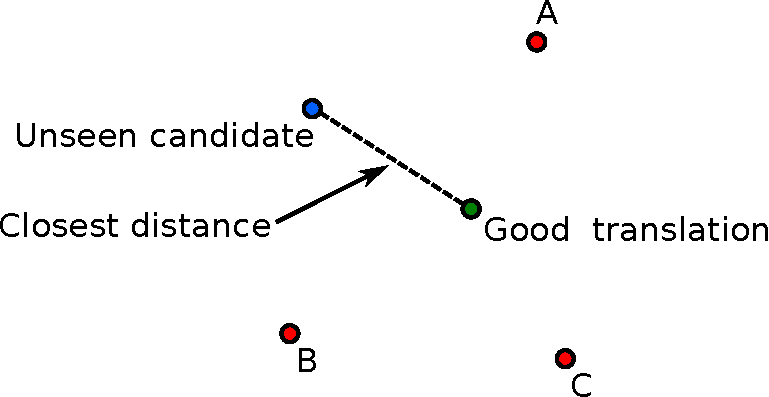
\includegraphics[width=8cm]{img/translation-space.pdf}
    \end{center}

    \caption[An illustration of a space of translations]{An example of a good
    translation with only a few candidate translations around it. If a number
  of dimensions is higher than the number of candidates it is intuitively quite
probable that the closest point to a new unseen candidate is the good
translation.}
    \label{translation-space-illustration}
\end{figure}

The average edit distances vary a lot. Systems cu-bojar, cu-depfix and cu-funky
have very low AED (0.2 --- 1.7), because they are very similar to each other.
Systems CU-TectoMT, onlineA and onlineB are in the middle of the AED range (3.1
--- 3.9) and since they are quite solitary in the set of ranked systems we can
consider their AEDs as representative values.  Systems commercial1 and
commercial2 have the highest AEDs. This could be explained by the fact that
both of the systems are rule based and produce dissimilar translations to those
generated by the statistical based systems. It is, however, interesting that
their translations are not even similar to each other. You can see the distribution of the absolute
counts with respect to the edit distance plotted in Figure
\ref{absolute-counts-per-distance}.

\begin{figure}
    \begin{center}
        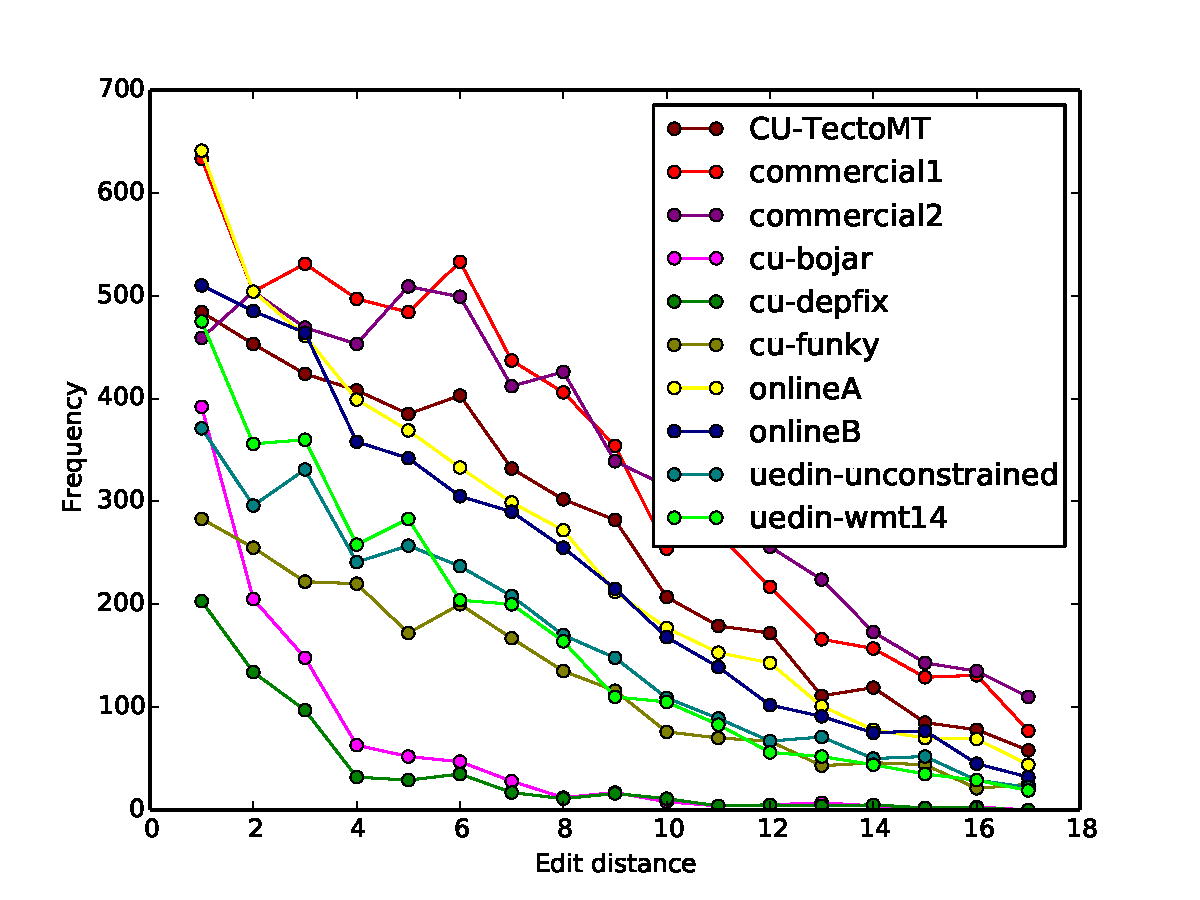
\includegraphics[width=14cm]{img/absolute-counts-per-distance.pdf}
    \end{center}

    \caption[Absolute counts of matched segments with respect to the edit distance]
    {Absolute counts of segments with respect to the edit distance}

    \label{absolute-counts-per-distance}
\end{figure}


To support the above statement (that the closest segment to an unseen candidate
is more likely to be of better quality) we have performed the following
analysis: For each left-out system we computed how often the closest segment
has better, equal or worse rank than the ``unseen'' segment (We can actually do
that, because we know the true rank of the segment removed from the database).
We computed these relative frequencies only on the missed segments (the closest
segment was not the same segment). You can see this analysis performed for the
individual systems in Table \ref{edit-distance-matching-analysis}.  You can
also see how these relative frequencies change with with a change of the edit
distance in Figure \ref{better-worse-equal-with-edit-distance}. More than a
half of the closest segments has better rank than the original segments and
only 20.6 \% of the segments have the same rank. This is really very poor
because it means that our approximation method which ranks unseen translations
has the accuracy only 20.6 \%. This accuracy does not differ much for
individual systems but there is an expected trend of similar systems (cu-bojar,
cu-depfix) having this accuracy slightly higher. 

As you can see in Figure \ref{better-worse-equal-with-edit-distance} the
relative number of closest systems which are ranked better grows quite
significantly with the edit distance. The relative number of the worse segments
is quite stable (around 0.3) and does not change significantly with the edit
distance. The relative number of closest segments which are equally raked as
the source segment is decreasing with the edit distance. For example, for the
segments whose edit distance to the closest segment is 17, only 10 percent of
the closest segments is equally ranked, which is really poor. 


\begin{table}
  \centering
\begin{tabular}{|lrrr|}
  \hline
  \textbf{Unseen system}            &   \textbf{Worse} &   \textbf{Equal} &   \textbf{Better} \\
  \hline
   commercial1         &   27.9 \% &   19.0 \% &    53.1 \% \\
   commercial2         &   23.3 \% &   17.5 \% &    59.2 \% \\
   cu-bojar            &   22.5 \% &   31.5 \% &    46.0 \% \\
   cu-depfix           &   32.7 \% &   33.2 \% &    34.0 \% \\
   cu-funky            &   28.8 \% &   23.8 \% &    47.4 \% \\
   CU-TectoMT          &   25.8 \% &   18.6 \% &    55.6 \% \\
   onlineA             &   28.1 \% &   20.4 \% &    51.5 \% \\
   onlineB             &   33.3 \% &   20.9 \% &    45.8 \% \\
   uedin-unconstrained &   32.4 \% &   22.3 \% &    45.3 \% \\
   uedin-wmt14         &   31.6 \% &   23.4 \% &    45.1 \% \\
  \hline
   All               &   28.1 \% &   20.6 \% &    51.2 \% \\
  \hline
\end{tabular}

\caption[Comparisons of unseen and the closest systems]{Comparisons of unseen
and the closest system. This table shows how often the closest segment in the
database was worse, equally good or better than the original ``unseen''
segment. These relative frequencies were computed only on missed segments
(which weren't already in the database).}

  \label{edit-distance-matching-analysis}
\end{table}

\begin{figure}
    \begin{center}
        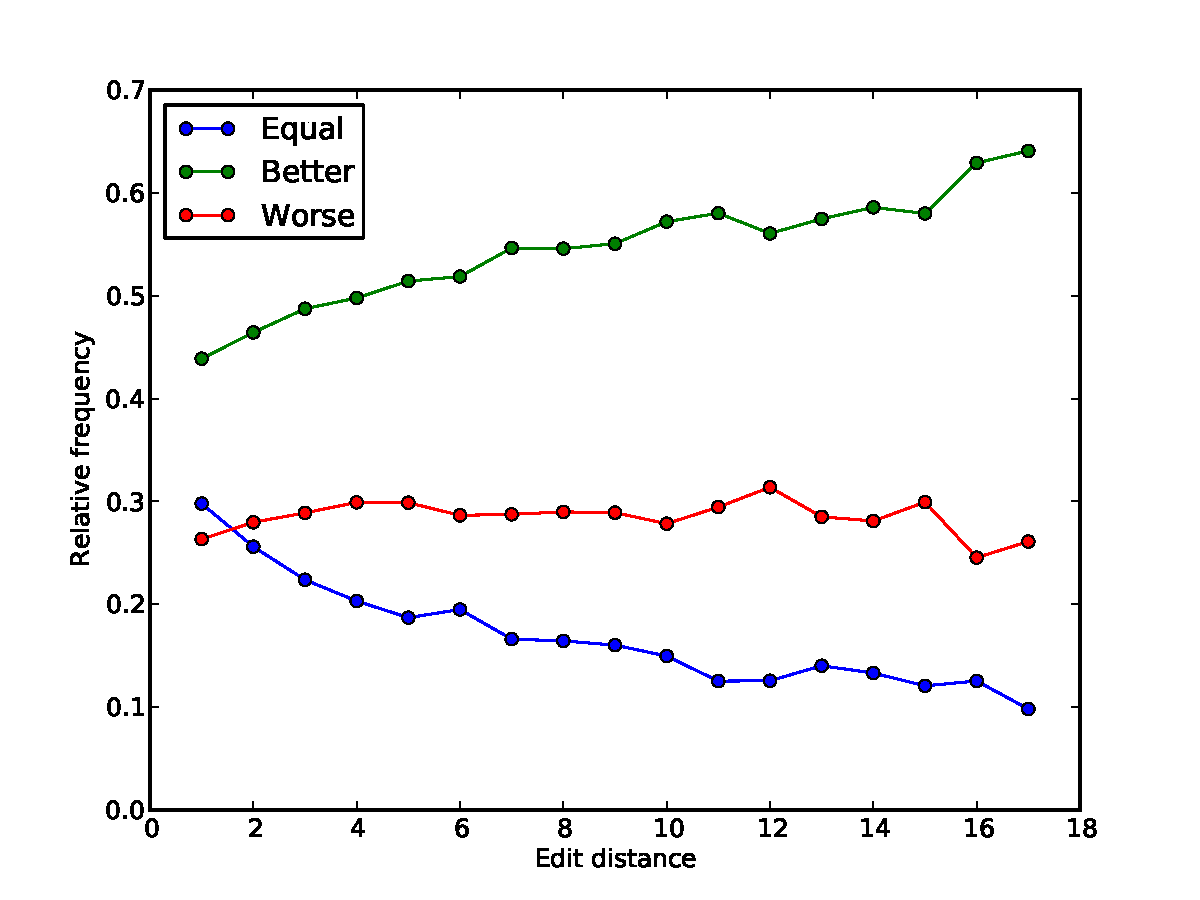
\includegraphics[width=14cm]{img/per-distance.pdf}
    \end{center}

    \caption[Comparisons of unseen and the closest systems with respect to the
    edit distance]{Comparisons of unseen and the closest systems with respect
    to the edit distance. The results in this figure are computed on all the
systems.}

    \label{better-worse-equal-with-edit-distance}
\end{figure}




We also listed a few example candidate segments in Table
\ref{segments-closest} together with the corresponding closest segments from
the database and their distances. We also report whether the closest segment
was ranked better, equal or worse than the ``unseen'' one.

\begin{table}
  \begin{center}
    \begin{tabular}{|p{5.5cm}p{5.5cm}rc|}
      \hline
      \textbf{Unseen segment} & \textbf{Closest segment} & \textbf{D} & \textbf{C} \\
      \hline
      s dokumenty upřednostňujícím doprovodem hradu & se dokumenty favorizovat doprovod hradu & 18 & \worse{} \\ \hline
      ze 120 domova m2 & z 120 m2 domova & 7 & \better{} \\ \hline
      vaše ústa ohřívá protein & vaše ústa zahřívání bílkovin & 10 & \better{} \\ \hline
      videokonference & videokonferenci & 1 & \better{} \\ \hline
      popřel užívání kokainu a & popřela užívání kokainu a & 1 & \worse{} \\ \hline
      přibližně šedesát- drah kilometru & přibližně šedesát-dráha kilometru & 3 & \equal{} \\ \hline
      v Liverpoolském porotním soudu & Liverpool Korunního soudu & 11 & \better{} \\ \hline
      je nesmysl v gravitaci filmu & Je nesmysl ve filmu gravitace & 15 & \better{} \\ \hline
      Pak 64,23 \% oprávněných voličů & pak 64,23 \% oprávněných voličů & 1 & \better{} \\ \hline
      podle DPA agentury & podle DPA agentury té & 3 & \worse{} \\ \hline
    \end{tabular}
  \end{center}

  \caption[Example candidates and the closest segments]{ Example candidates and
    the closest segments. The last but one column (\textbf{D}) stands for
    distance and contains distances of the unseen candidates to the closest
    segments. The last column (\textbf{C}) stands for comparison; the closest
  segment is either worse (\worse{}), equally good (\equal{}) or better
(\better{}) than the original unseen segment.}

  \label{segments-closest}
\end{table}

We have to unfortunately conclude, that the proposed method, which reuses the
database for evaluating unseen translations, does not work. We analyzed the
results and the main cause of this failure seems to be that the systems tend to
agree on better translations and their translations tend to be more similar to
better translations in the database so we cannot predict their rank accurately. 

\subsection{Enhancing reference translation with good candidates from the database}
\label{enhancing:bleu}

Following the conclusions from the previous two subsections, it seems that
errors in machine translation are very unique. Any database of bad examples
(bad translations) is therefore very sparse. It is very well known fact that a
number of correct translations is very high \parcite{bojar2013scratching}. It
seems, however, that the number of bad translations is much higher and
therefore it make more sense to use a database of good translations. 

In the following experiment we therefore use only the good candidate segments
from the annotated database. The approach used here is, however, different from
the previous experiments. We would like to measure how similar are candidates
to the good translations from the database. This is very similar to what
automatic metrics do when measuring similarity between a candidate and a
reference translations. We have therefore decided to use one of the standard
metrics -- \metric{BLEU} -- to measure this similarity. First, we are going to
introduce the metric and then we are going to customize it for our experiment. 

\begin{table}
  \begin{center}
      \subfloat[\metric{SegRanksBLEU}, correlation: 0.9745 ]{
        \begin{tabular}{|l|c|}
          \hline
          \textbf{System} & \textbf{Score} \\
          \hline
          cu-depfix & 0.305 \\
          cu-funky & 0.302 \\
          uedin-unconstrained & 0.302 \\
          cu-bojar & 0.300 \\
          uedin-wmt14 & 0.296 \\
          onlineB & 0.289 \\
          onlineA & 0.259 \\
          CU-TectoMT & 0.225 \\
          commercial1 & 0.176 \\
          commercial2 & 0.160 \\
          \hline
        \end{tabular}
      \label{enhanced-bleu-results}
    }
    \,
    \subfloat[\metric{BLEU}, correlation: 0.9751]{
        \begin{tabular}{|l|c|}
          \hline
          \textbf{System} & \textbf{Score} \\
          \hline
          cu-depfix & 0.221 \\
          cu-bojar & 0.221 \\
          cu-funky & 0.221 \\
          uedin-unconstrained & 0.220 \\
          uedin-wmt14 & 0.215 \\
          onlineB & 0.207 \\
          onlineA & 0.187 \\
          CU-TectoMT & 0.157 \\
          commercial1 & 0.114 \\
          commercial2 & 0.102 \\

          \hline
        \end{tabular}
      \label{bleu-results}
    }

  \end{center}

  \caption[Overall system ranking according to \metric{SegRanksBLEU} and
  \metric{BLEU} scores]{Overall system ranking according to
  \metric{SegRanksBLEU} and \metric{BLEU} scores. Please see the chapter
  \ref{metrics} for the details of computation of the reported correlations.}

  \label{segranksbleu:experiment}
\end{table}

Metric \metric{BLEU} was developed by \perscite{Papineni02bleu:a} and it is the
most used metric in the machine translation evaluation. It is defined as the
geometric mean of n-gram precisions for $n \in \{1 \ldots N\}$, where $N$ is
usually 4. More precisely, for a candidate $c$ and reference translations $r_i$
where $i \in I$, let the clipped count of an n-gram $g$ be defined as follows:

\begin{equation*}
    \text{count}_{clip}(g,c,r) = \min \left( \cnt(g, c), ~ \max_{i \in I} \left( \cnt(g, r_i) \right) \right)
\end{equation*}

\noindent where $\cnt(g, s)$ denotes the count of n-gram $g$ in the sentence
$s$. The modified precision $p_n$ is then defined as:

\begin{equation*}
    p_n = \frac{
        \sum_{g \in \text{n-grams}(c)} \text{count}_{clip}(g,c,r)
    }{
        \sum_{g \in \text{n-grams}(c)} \cnt(g,c)
    }
\end{equation*}

\noindent Using the computed n-gram precisions, we can compute the final
\metric{BLEU} score:

\begin{equation*}
        BLEU = BP \cdot \exp \left( \frac{1}{N} \sum_{i = 1}^N \log p_n \right) 
\end{equation*}

\noindent where $BP$ is the brevity penalty (meant to penalize short outputs to
discourage improving precision at the expense of recall) defined as follows:

\begin{equation*}
    BP = \left\{ 
  \begin{array}{l l}
    1 & \quad \text{if } |c| > |r|\\
    \exp(1-|r|/|c|) & \quad \text{if } |c| \leq |r| \\
    \end{array} \right.
\end{equation*}

\noindent where $|c|$ and $|r|$ are the lengths of the candidate and reference
translations respectively. In the case of multiple reference translations,
$|r|$ could be the average length, the maximum length or the length closest to
the candidate $c$.

This experiment consists of two steps. In the first step we select good segment
translations from the short segments database. In the second step we use the
selected good segment translations to enhance reference translations when
computing \metric{BLEU}.

Since the assigned ranks in the database are relative, we cannot know which
segments are really good in the term of the absolute quality. We have to assume
that there is at least one good candidate translation among the ranked
candidates and consider all candidate segments with the best rank as the good
translations. We select these candidate segments for each source segment for
each sentence.

Finally, we use the selected good segments as the reference translations in
addition to the original reference sentence translated by human expert.  Since
the new references are only short segments and do not cover a whole sentence,
we use only the length of the original reference sentence in the computation of
the brevity penalty. To distinguish this method from the standard \metric{BLEU}
with the single official reference translation, we will call this method
\metric{SegRanksBLEU}.

Please note, that introducing the new reference
translations, which do not change the brevity penalty, can only increase the
clipped counts of n-grams occurring in the short segments.  Candidates will be
rewarded for having n-grams which are also in the good segment translations in
the database.

You can see the overall rankings of the evaluated systems as given by
\metric{SegRanksBLEU} and \metric{BLEU} in Table
\ref{segranksbleu:experiment}. As expected, the \metric{SegRanksBLEU} scores
are really much higher than \metric{BLEU}. However, the reported system level
correlations of these two metrics are almost equal (correlation of
\metric{SegRanksBLEU} is even a little bit lower).  \XXX{Jak tohle zanalyzovat
a vysvetlit?}


\section{Tuning Systems}
\label{tuning-systems}

Automatic metrics are not used only for evaluating already developed systems on
test sets. They are also often used when tuning a system to choose the
parameters of a model which gives the best metric score computed on a
development test set. One of the methods utilizing automatic metrics for system
tuning is Minimum Error Rate Training (MERT). We will describe the theory
behind the MERT in the following subsection a then we will experiment with
using the short segments rank database in the MERT.

\subsection{Minimum Error Rate Training}

Most of the statistical machine translation systems model the posterior
probability of producing a sentence translation $e$ given a source sentence $f$
using a log-linear model \parcite{Och:2002}: 

\newcommand{\vect}[1]{\boldsymbol{#1}}
\begin{equation}
    P(e \mid f) = %p_{\lambda_1^M} (e \mid f) =
    \frac
        {\exp \left(\sum_{m=1}^M \lambda_m h_m(e,f) \right)}
        {\sum_{e'} \exp \left(\sum_{m=1}^M \lambda_m h_m(e',f)\right)}
    = \frac
    {\exp \left( \vect{\lambda} \cdot \vect{h}(e,f)  \right)}
    {\sum_{e'} \exp \left(\vect{\lambda} \cdot \vect{h}(e',f)\right)}
\end{equation}

\noindent where the vector $\vect{h}(e,f) = \{ h_1(e,f), h_2(e,f), \ldots ,
h_M(e,f) \}$ is a feature vector and the vector $\vect{\lambda} = \{\lambda_1,
\lambda_2, \ldots, \lambda_M \}$ is a feature weight vector. It can be easily
shown that when searching for the best candidate $e_{best}$, the above
log-linear formula could be simplified to the following:

\begin{equation}
  e_{best}  =  \argmax_e \left\{ P(e \mid f) \right\}
  =  \argmax_e \left\{ \vect{\lambda} \cdot \vect{h}(e,f) \right\}
\end{equation}

Now the problem with this log-linear model is how to find the weight vector
$\vect{\lambda}$ which would give the best translations. And this is what the
MERT method solves.

Let $F = \{f_i;~ i \in I\}$ be a held out corpus in the source language and $R
= \{r_i;~ i \in I\}$ be a corresponding reference translation. Traditionally
the best weight vector $\vect{\lambda}$ can be found using the maximum
likelihood principle:

\begin{equation}
  \vect{\hat\lambda} = \argmax_{\vect{\lambda}} \left\{ \prod_{i \in I}
  P_{\vect{\lambda}} (e_i \mid f_i ) 
\right\}
\end{equation}

\noindent This optimization problem has some very nice properties: there is
one global optimum and there are algorithms which converge to this optimum.
\perscite{Och:2003}, however, argues that that there is no proof that this
method gives the best weights with respect to the translation quality. 

He suggested to choose the weight vector $\vect{\lambda}$ which produces the
best translation of the heldout data. We can measure the quality of the
translation using an automatic metric $m(E,R)$, where $E$ is the set of
candidate translations produced by the MT system and $R$ is a set of reference
translation. We are therefore going to minimize the score (or minimize it in
the case the metric is error based and returns lower scores for better
translations) of the metric:

\begin{equation}
  \vect{\hat\lambda} = \argmax_{\vect{\lambda}} \left\{ m( \hat{E}(F,
  \vect{\lambda}), R ) \right\}
    \label{eq:errorrate-opt}
\end{equation}

\noindent where $\hat{E}(F, \vect{\lambda})$ is the corpus $F$ translated with
the weights $\vect{\lambda}$ and $\hat{e}(f, \vect{\lambda})$ is the
translation of a sentence $f$ with weights $\vect{\lambda}$:

\begin{equation}
  \hat{E}(F, \vect{\lambda}) = \left\{ \hat{e}(f_i, \vect{\lambda});~i \in I\right\}
    \label{eq:corpus-translation}
\end{equation}

\begin{equation}
  \hat{e}(f, \vect{\lambda}) = 
    \argmax_{e} \left\{ \vect{\lambda} \cdot \vect{h}(e, f) \right\}
    \label{eq:sentence-translation}
\end{equation}

The criterion \eqref{eq:errorrate-opt} is, however, not so easy to optimize. It
contains argmax operation and therefore it is not smooth and it is not possible
to use a gradient based method. It has also a lot of local maximums.
\perscite{Och:2003} therefore suggested to use Powell's algorithm
\parcite{Powell:1964} which does not need gradient to optimize a function.

In each step, Powell's algorithm starts at a point from which it goes in
several directions (possibly also in random directions) and optimizes the
function along the lines which originate at the start point using a given line
optimization method. The most optimal point found on the lines is then used as
the new starting point in the next step. 

The Powell's algorithm depends on an efficient line optimization method. Och
proposed a method which takes advantage of log-linear model properties. In the
following we limit the space of the optimization problem to a line defined by
the following equation:

\begin{equation}
  \vect{\lambda}(\gamma) = \vect{\lambda'} + \gamma \vect{d}
  \label{eq:line}
\end{equation}

\noindent where $\vect{\lambda'}$ defines a starting point and the vector
$\vect{d}$ defines a direction of the line. Now, we can reformulate the limited
optimization problem:

\begin{equation}
  \hat{\gamma} = \argmax_{\gamma \in \mathbb{R}} \left\{ m(\hat{E}(F,\vect{\lambda}(\gamma)),R) \right\}
    \label{eq:line-opt}
\end{equation}

When we apply the line equation \ref{eq:line} in the argmax operator which
choose the best translation in the equation \ref{eq:sentence-translation}, we
get the following.

\begin{eqnarray}
  \hat{e}(f, \vect{\lambda}(\gamma))
    & = & \argmax_{e} \left\{ \vect{\lambda}(\gamma) \cdot  \vect{h}(e, f) \right\} \\
    & = & \argmax_{e} \left\{ \vect{\lambda'} \cdot \vect{h}(e, f) + \gamma \vect{d} \cdot \vect{h}(e, f) \right\} \\
    & = & \argmax_{e} \left\{ t(e,f) + \gamma \cdot m(e,f) \right\} \label{eq:argmax}
\end{eqnarray}

\noindent where the scalars $t(e,f)$ and $m(e,f)$ are constant for a given
candidate $e$. This means, that each candidate $e$ specifies a line given by
the equation $x = t(e,f) + \gamma \cdot m(e,f)$ which computes the candidate
score for the parameter $\gamma$. The argmax operator in the equation
\eqref{eq:argmax} then choose the candidate whose line is the highest in a
given $\gamma$. You can see this situation illustrated in Figure
\ref{fig:lines}.  The line optimization method finds all the intersections of
the lines where the best candidate (with the highest model score) changes. The
intersections found for each sentence in the heldout data are then merged to
obtain intervals of $\gamma$ in which the $\gamma$ does not change the set of
the highest score candidates.  For each interval, the metric score is computed
and the optimal $\gamma$ is chosen from the interval with the highest metric
score. Since the metrics are often computed from sentence decomposable
statistics, we can easily update the metric's score in each interval boundary
by subtracting the old sentence's statistics and adding the new sentence's
statistics.

\begin{figure}
    \begin{center}
        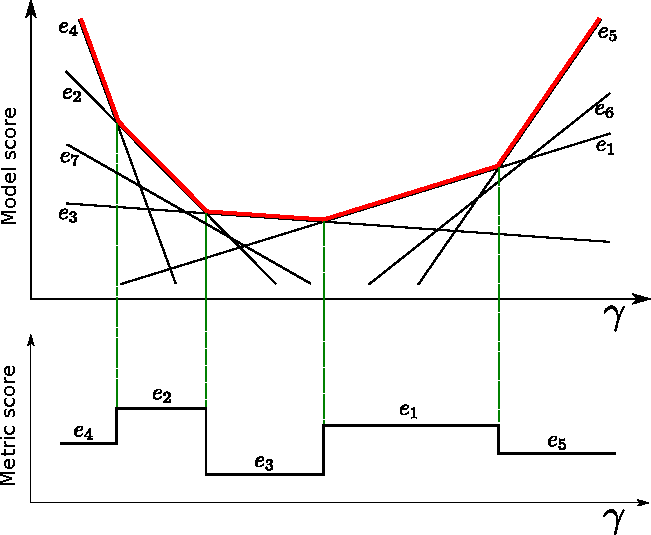
\includegraphics[width=10cm]{img/mert.pdf}
    \end{center}

    \caption[An illustration of the line optimization in MERT]{
      An illustration of the line optimization in MERT. You can see two sentences and their
      candidate translations represented by the lines. The best candidate in each interval
      is marked by the red line. The bottom part of the figure illustrates how the metric score
      depends on $\gamma$.
}

    \label{fig:lines}
\end{figure}

The last difficulty in the MERT method is that we cannot easily enumerate all
the candidate sentences. For that reason the n-best list approximation is used:
the decoder produce $n$ best translations for each sentence and only these $n$
translations are considered during the optimization. A problem arise when the
optimal weight vector found during the optimization gets too far from the
weight vector used to produce the initial n-best list. For that reason a new
n-best list is produced with the new weights, it is merged with previous n-best
lists and optimization process is run again in new MERT iteration. When the
optimal weight vector converges or a maximum number of iterations is reached
the MERT method ends. 

\subsection{Experiments with MERT}

MERT method is most often used with BLEU metric even it does not have the best
correlation with human judgments (see the chapter \ref{metrics} for more
details). However, there is a lot of experiments with utilizing also other
automatic metrics in recent time. In WMT11 \parcite{wmt11}, there was a shared
task in which participants tuned a common system with different metrics. The
tuned systems were then evaluated by humans and some of them outperformed the
baseline system tuned with BLEU.

It is not feasible to employ any sort of human evaluation directly in the MERT
process. On the one hand human evaluation is very slow and expensive, on the
other hand MERT requires to evaluate very long n-best list in each iteration.
There are some suggestions to do the manual evaluation in a clever way and
lower the amount of manual work. For example \perscite{human-in-the-loop}
noticed that a lot of short segments is repeated in a n-best list and therefore
suggest to extract these short segments from a n-best list in each MERT
iteration and let humans rank them. (Actually our short segment extraction
method was partially inspired by this work). However they did not try this
method in an actual MERT run yet for lack of resources. 

We believe that a much less expensive way to introduce an element of human
evaluation in MERT method is to use some sort of semi-automatic metric in which
a certain amount of manual work is needed at the beginning and then the metric
evaluates translations automatically. In this subsection, we therefore
experiment with previously introduced metrics which rely on the collected
database of short segment ranks.

\subsubsection{Tuned System}

The system we tried to tune is the system cu-bojar \parcite{tamchyna2014},
which we also used previous sections as one of the evaluated systems. This
system is Moses-based and combines several different approaches:

\begin{itemize}
  \item factored phrase-based Moses model
  \item domain-adapted language model
  \item deep-syntactic MT system TectoMT
\end{itemize}

The parallel data used to train the phrase tables consists of 14.83 million
parallel sentences taken from the CzEng corpus \parcite{bojar:czeng} and 0.65
millions of sentences taken from the Europarl corpus \parcite{koehn:europarl}.
The monolingual data used to train language models consists of 215.93 million
sentences taken from the Czech side of the CzEng corpus and from 5 sources of
news domain. 

They used their baseline systems to translate WMT test sets from years
2012--2014.  These translation were then used to retrieve similar Czech
sentences using information retrieval techniques which were then used to train
the domain-adapted language model.

The deep-syntactic MT system TectoMT was used to translate WMT test sets from
years 2007--2014. These new synthetic parallel training data were then used to 
train an additional phrase table. 

Please note that both the domain-adapted language model and the TectoMT phrase
table were also trained on the data we use as development set and test set so
that tuning can assign appropriate weights to them.

There is 15 component weights to tune in total. \perscite{tamchyna2014} of
course tuned their system cu-bojar when participating in the translation shared
task but we use their system before it was tuned by them to tune it ourselves. 

We used the implementation of MERT which is distributed with Moses
toolkit\footnote{\url{http://www.statmt.org/moses/}}. It is implemented in C++
and new metrics are created by subclassing the base \pojem{Scorer} class. Since
the annotated database is stored in Python data structures and since a
development in Python is much easier and faster, we have implemented new
\pojem{PythonScorer} which is an universal wrapper around an arbitrary Python
scorer class, implemented using the Python C API.


\subsubsection{Metric Variants}

Our original idea was that we will use the alignment produced by the Moses
decoder during translating the n-best list to project the extracted short
source segments to the target side to have candidates which would be extracted
the same way as the ranked segments in the database. Unfortunately the
alignment produced by Moses decoder is very sparse and unreliable (which may be
caused by a bug in the code) so we had to get along without the alignment.

The naive approximation is to just test whether the ranked candidate segments
from the database also occurs in evaluated sentences. The first metric we use
in MERT experiment is therefore very similar to the \metoda{Exact Matching}
method in Section \ref{exact:matching}. For each ranked source segment we
test if any of its candidate segment occurs in the evaluated sentence. If it
does we extract all pairwise comparisons inferred from the matched segment. If
more candidate segments occurs in the evaluated translation, we choose the
longest segment (assuming that the sorter segments are just substring of the
longest one). The final score is then computed as \metoda{Ratio of wins
(ignoring ties)}. We call this metric \metric{ExactMatch} in the following.

Even if the hit rate (percentage of segment candidates which are already ranked
in the database) computed on a whole n-best list would be 100 \%, the
\metric{ExactMatch} metric still does not evaluate whole sentences and could be
too coarse and harsh. Moreover, if the hit rate drops during the tuning, the
metric score would be computed on a very small percentage of development set
and would be very unstable. To ensure the tuning is stable, we interpolate all
the metrics in this section (if not said otherwise) together with BLEU with
equal weights. We also tried to tune using the \metric{ExactMatch} metric
solely but the tuned system translated very badly and the hit rate dropped very
low during the tuning. We could explain this by that the system was tuned to
translate a few ranked segments well (so these segments were hits) but other
segments were missed and translated badly. The optimal metric score was
therefore computed on a very small fraction of the development set and did not
reflect the overall quality of the translation.

Since we do not have the alignment and cannot extract the candidate segments
exactly, we unfortunately cannot use the method introduced in Subsection
\ref{match:editdistance} which matches the closest segment in the database by
edit distance.  To avoid the shortcomings of the \metric{ExactMatch} metric
(the metric is not computed on all the extracted source segments and an unseen
system is more likely to cause hit in the database with better translations) we
propose another variant called \metric{PenalizeUnknown}. This variant differs
to \metric{ExactMatch} in that it considers all missed segments as the worst
translations. We agree that the assumption that all unseen and unranked
segments are wrong is not correct, but this approach could increase the hit
rate. The question is then, whether we prefer to have a system which produces a
lot of segments which were already ranked (even badly) or a system which
produces a lot of unranked segments which we hope to be of better quality.

The last variant we experiment with is \metric{SegRanksBLEU} metric introduced
in Subsection \ref{enhancing:bleu}. Because this metric is already based on
BLEU metric (and use the reference translation) we do not interpolate it with
BLEU anymore.


\subsubsection{Results and Analysis}

You can see the results of the tuned system in Table \ref{mert:results}. We
used the tuned systems to translate the test set (newstest2012) and then we
evaluated these translations automatically and manually. For the automatic
evaluation we used metrics \metric{BLEU} \parcite{Papineni02bleu:a} and
\metric{CDER} \parcite{Leusch06cder:efficient}. We have also conducted a small
scale manual evaluation. For each evaluated system, we randomly sampled
\XXX{100} sentences which were translated differently by the baseline and by
the evaluated system. \XXX{Two} annotators then compared the sampled
sentences with the corresponding translations produced by the baseline system.
Their task was to choose which sentence is better or whether they are of the
same quality. We report how many of the sampled sentences were better and
better-or-equal than the corresponding baseline translation.

You can see that none of the metric variants outperformed the baseline system
tuned solely to \metric{BLEU} in the automatic evaluation.

\begin{table}
  \centering
  \begin{tabular}{|r|c|cc|cc|}
    \hline
    & \textbf{\#Mert} & \multicolumn{2}{|c|}{\textbf{Automatic}} & \multicolumn{2}{|c|}{\textbf{Manual}} \\
    & \textbf{iter-} & \multicolumn{2}{|c|}{\textbf{Evaluation}} & \multicolumn{2}{|c|}{\textbf{Evaluation}} \\
    \textbf{Tunable metric} & \textbf{ations} & \textbf{BLEU} & \textbf{CDER}  & \textbf{Better} & \textbf{Worse} \\
    \hline
    \metric{BLEU} (baseline) & 11 & 0.1782 & 0.3855 & --- & --- \\
    \metric{ExactMatch}      & 20 & 0.1637 & 0.3674 & \XXX{} & \XXX{} \\
    \metric{PenalizeUnknown} &  8 & 0.1772 & 0.3850 & \XXX{} & \XXX{} \\
    \metric{SegRanksBLEU}    &  8 & 0.1753 & 0.3835 & \XXX{} & \XXX{} \\
    \hline
  \end{tabular}

  \caption[Results of systems tuned on SegRanks based metrics]{Results of
    systems which were optimized to a SegRanks based metric. The items in the
    first column specify the metric which was used when tuning the system on
    the development test.  The columns BLEU and CDER contain just scores of
    these metrics computed on the test set translated with the tuned weights.
  The last two columns contain percentages of better and better-or-equal
sentences compared to the baseline in the manual evaluation.}

  \label{mert:results}
\end{table}

\XXX{Okomentovat vysledky, az budou vsechny a hlavne az bude lidske hodnoceni}


\begin{figure}
    \begin{center}
        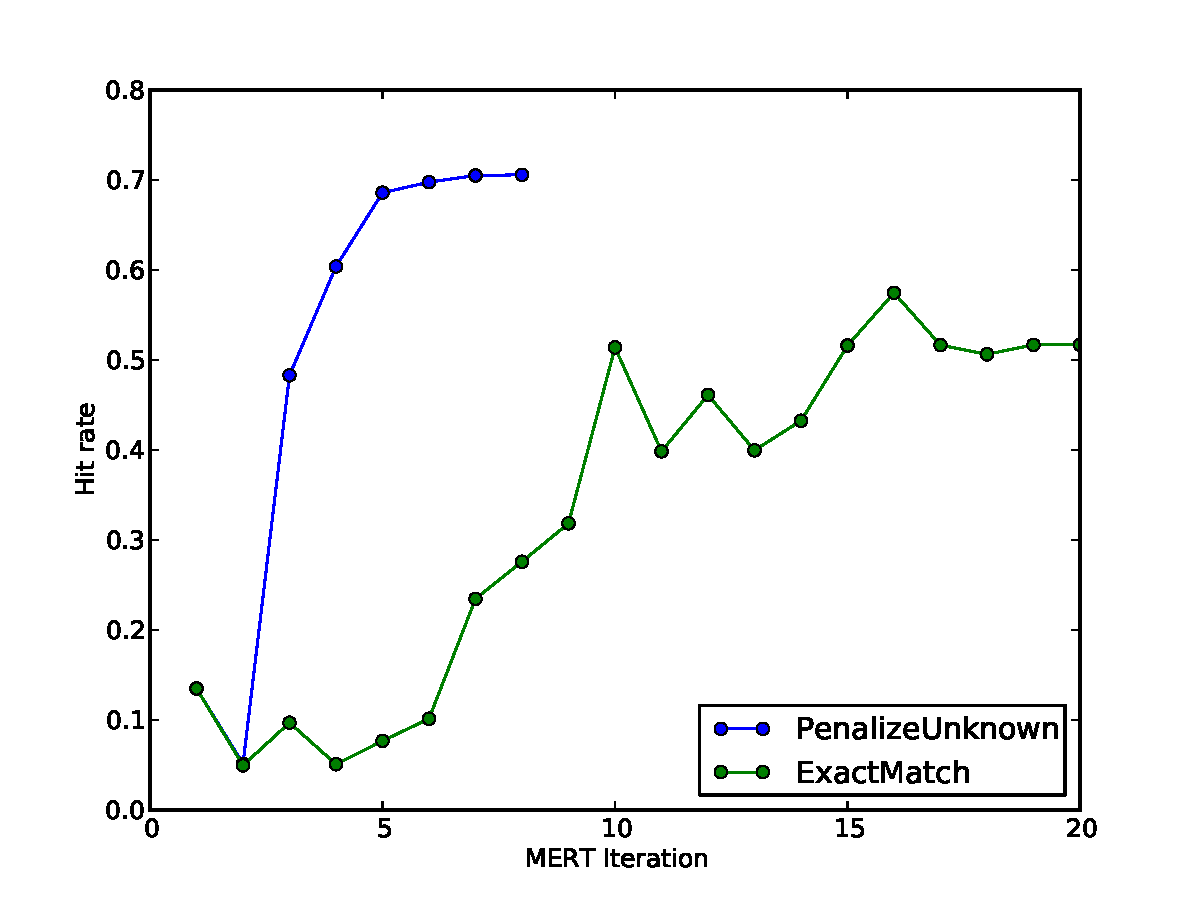
\includegraphics[width=12cm]{img/hit-rates-plot.pdf}
    \end{center}

    \caption[Hit rates computed on the n-best lists produced in MERT]{Hit rates
    computed on the n-best lists produced in each MERT iteration}

    \label{hit:rates:plot}
\end{figure}


To see the differences between \metric{ExactMatch} and
\metric{PenalizeUnknown}, we have plotted the values of hit rates computed in
each MERT iteration in Figure \ref{hit:rates:plot}. You can see that
\metric{PenalizeUnknown} gets to the hit rate 0.7 very quickly (in the sixth
iteration) and its growth is quite stable. This is however expected, since the
objective function also indirectly optimizes the hit rate. The hit rate in
\metric{ExactMatch} also grows but much more slowly. It stabilizes around the
value 0.5. The good point is that the final value is quite high so the
\metric{ExactMatch} is computed on nonnegligible amount of data. However, it
takes much more iterations for \metric{ExactMatch} to get to the value 0.5 that
it takes for \metric{PenalizeUnknown} to get to the value 0.7. \XXX{Tady to jeste
shrnout po manualni evaluaci}.




\XXX{Je otaka, zda jsme se podle Penalize Unknown nedostali k puvodnimu systemu}

\chapter{Evaluation and Comparison of Automatic Metrics}
\label{metrics}

% \XXX{Pretavit abstrakt do nejakeho uvodu}
%
% Puvodni abstrakt, neco z toho dat do vlastniho abstraktu
%
% This paper presents the results of the WMT14 Metrics Shared Task. We asked
% participants of this task to score the outputs of the MT systems involved in
% WMT14 Shared Translation Task. We collected scores of 23 metrics from 12
% research groups. In addition to that we computed scores of 6 standard metrics
% (BLEU, NIST, WER, PER, TER and CDER) as baselines. The collected scores were
% evaluated in terms of system level correlation (how well each metric's scores
% correlate with WMT14 official manual ranking of systems) and in terms of
% segment level correlation (how often a metric agrees with humans in comparing
% two translations of a particular sentence).

Automatic machine translation metrics play a very important role in the
development of MT systems and their evaluation. There are many different
metrics of diverse nature and one would like to assess their quality. For this
reason, the Metrics Shared Task is held annually at the Workshop of Statistical
Machine Translation\footnote{\url{http://www.statmt.org/wmt13}}, starting with
\perscite{koehn-monz:2006:WMT} and following up to
\perscite{wmt14-overview-paper}. In WMT13, we took over the organization of the
task \parcite{machacek:2013} and continued to do that also in WMT14
\parcite{machacek:2014}. In this chapter, we present the results of WMT14
metrics shared task with some additional information and comments.

In this task, we asked metric developers to score the outputs of WMT14 Shared
Translation Task \parcite{wmt14-overview-paper}. We have collected the computed
metrics' scores and use them to evaluate the quality of the metrics.  There are
actually two subtasks: a system level task and a segment level task.

\begin{itemize}

    \item \textbf{System Level.} In the system level subtask, participants
        compute one score for the whole test set, as translated by each of the
        systems. We then measure the correlation of those scores with the systems'
        official human scores.  The goal of metrics in this subtask is to give
        an overall ranking of the systems as close as possible to the official
        ranking according to human scores in each direction.
    
    \item \textbf{Segment Level.} In this subtask, participants compute one
        score for each sentence of each system's translation. We then measure
        the correlation of these scores with pairwise human judgements. The
        goal of metrics in this subtask is to compare two candidate segments in
        the same way as humans would.

\end{itemize}

In the previous years, a lot of metrics performed very well in the system level
task. In some of the translation directions, they predicted the overall ranking
of systems almost perfectly. However, there is still space for metrics to
improve.  In contrast to the system level task, the segment level task is much
more difficult. The correlations in previous years were very low. It is
therefore very interesting to see whether metrics perform better this year.

The systems' outputs, human judgements and evaluated metrics are summarized in
Section \ref{section:data}. In Section \ref{section:metrics:description}, we
describe the participated metrics in more detail. The quality of the metrics in
terms of system level correlation is reported in Section \ref{system-level}.
The Segment level correlation with a detailed discussion and a slight change in
the calculation compared to the previous year is reported in Section
\ref{segment-level}.

\section{Data}
\label{section:data}

We used the translations of MT systems involved in WMT14 Shared Translation
Task together with reference translations as the test set for the Metrics Task.
This dataset consists of 110 systems' outputs and 10 reference translations in
10 translation directions (English from and into Czech, French, German, Hindi
and Russian). For most of
the translation directions each system's output and the reference translation
contain 3003 sentences. For more details please see the WMT14 overview
paper \parcite{wmt14-overview-paper}. 

\subsection{Manual MT Quality Judgements}

During the WMT14 Translation Task, a large scale manual annotation was conducted
to compare the systems. We used these collected human judgements for the evaluation
of
the automatic metrics. 

The participants in the manual annotation were asked to evaluate the system outputs
by ranking translated sentences relative to each other. For each source segment
that was included in the procedure, the annotator was shown the outputs of five
systems to which he or she was supposed to assign ranks. Ties were allowed.

These collected rank labels for each five-tuple of systems were then interpreted
as 10 pairwise comparisons of systems and  used to assign each system a score
that
reflects how high that system was usually ranked by the annotators. Please see
the WMT14 overview paper for details on how this score is computed. You
can also find inter- and intra-annotator agreement estimates there.


\subsection{Participants of the Metrics Shared Task}

\begin{table*}[t]
  \small
  \begin{center}
    \begin{tabular}{rl}
      \textbf{Metric} & \textbf{Participant} \\
      \hline
      \metric{AMBER} & National Research Council of Canada \parcite{improving:amber} \\
      \metric{APAC} & Hokkai-Gakuen University \parcite{wmt14-metric-apac} \\
      \metric{BEER} & ILLC -- University of Amsterdam \parcite{wmt14-metric-beer} \\
      \metric{BLEU-NRC} & National Research Council of Canada \parcite{wmt14-metric-bleunrc} \\
      \metric{DiscoTK-*} & Qatar Computing Research Institute \parcite{wmt14-metric-discotk} \\
      \metric{ELEXR} & University of Tehran \parcite{wmt14-metric-elexr} \\
      \metric{LAYERED} & IIT, Bombay \parcite{wmt14-metric-layered} \\
      \metric{Meteor} & Carnegie Mellon University \parcite{wmt14-metric-meteor} \\
      \metric{Parmesan} & Charles University in Prague \parcite{wmt14-metric-parmesan} \\
      \metric{RED-*} & Dublin City University \parcite{wmt14-metric-red} \\
      \metric{tBLEU} & Charles University in Prague \parcite{wmt14-metric-tbleu} \\
      \metric{UPC-IPA} & Technical University of Catalunya \parcite{wmt14-metric-upc} \\
      \metric{UPC-STOUT} & Technical University of Catalunya \parcite{wmt14-metric-upc} \\
      \metric{VERTa-EQ} & University of Barcelona \parcite{wmt14-metric-verta} \\
      \metric{VERTa-W} & University of Barcelona \parcite{wmt14-metric-verta} \\
    \end{tabular}
  \end{center}
  \caption{Participants of WMT14 Metrics Shared Task}
  \label{participants}
\end{table*}

Table \ref{participants} lists the participants of WMT14 Shared Metrics Task,
along with their metrics. We have collected 23 metrics from a total of
12 research groups.

In addition to that we have computed the following two groups of standard
metrics as baselines: 

\begin{itemize}

\item \textbf{Mteval.} The metrics \metric{BLEU} \parcite{Papineni02bleu:a} and
    \metric{NIST} \parcite{Doddington:2002:NIST} were computed using the script
    \texttt{mteval-v13a.pl}\footnote{\url{http://www.itl.nist.gov/iad/mig//tools/}}
    which is used in the OpenMT Evaluation Campaign and includes its own
    tokenization.  We run \texttt{mteval} with the flag
    \texttt{-{}-international-tokenization} since it performs slightly better
    \parcite{machacek:2013}.

\item \textbf{Moses Scorer.} The metrics \metric{TER} \parcite{Snover06astudy},
    \metric{WER}, \metric{PER} and \metric{CDER} \parcite{Leusch06cder:efficient}
    were computed using the Moses scorer which is used in the Moses model
    optimization. To tokenize the sentences we used the standard tokenizer
    script as available in the Moses toolkit.


\end{itemize}

We have normalized all metrics' scores such that better translations get higher scores. 

\section{Descriptions of the Metrics}
\label{section:metrics:description}

In this section, we present short descriptions of some interesting metrics which
participated in the shared task.  Please see the cited papers for more details
about the metrics. Note that the description of the \metric{BLEU} metric
has been already presented in Subsection \ref{enhancing:bleu}.

\subsection{AMBER}

Metric \metric{AMBER} is developed by \perscite{improving:amber}. The abbreviation 
stands for ``A Modified Bleu, Enhanced Ranking metric''. This metric is based
on \metric{BLEU} metric because, as the authors explain, \metric{BLEU}

\begin{itemize}
    \item is language independent,
    \item can be computed quickly (important for tuning),
    \item seems to be the best tuning metric.
\end{itemize}

\noindent They want to improve the correlation with human judgments while
preserving the advantages which make \metric{BLEU} so popular.
The basic formula for this metrics follows:

\begin{equation*}
    AMBER = score \cdot penalty
\end{equation*}

\noindent where $penalty$ is a weighted geometric average of 10 various penalty
measures and $score$ is given by:

\begin{equation*}
    score  = \theta_1 \cdot AvgP
           + \theta_2 \cdot Fmean 
           + \theta_3 \cdot AvgF 
\end{equation*}

\noindent where $AvgP$ is a geometric average of n-gram precisions (this is the
same as in \metric{BLEU}), $Fmean$ is the F-measure computed on the average
n-gram precision and average n-gram recall (averages are computed across $n \in
\{1, \ldots, N\}$) and $AvgF$ is an average (across $n \in \{1, \ldots, N\}$)
of F-measures computed on n-gram precision and n-gram recall for given $n$.

This is the basic computation but the authors propose many more enhancements,
for example they propose 8 different preprocessing (normalization and
tokenization) methods which are used to compute \metric{AMBER} metric on each
method separately and then return the average of scores computed after applying
all the methods. All free parameters of this metric were manually tuned on a
development set.

While we agree that the authors managed to preserve the key properties of
\metric{BLEU} mentioned above, we think that one of the most popular properties
of \metric{BLEU} is its implementation simplicity which is definitely not
preserved in \metric{AMBER}. 

\subsection{BEER}

This metric is proposed by \perscite{wmt14-metric-beer}. The abbreviation
stands for ``BEtter Evaluation as Ranking''. Their metric model can employ
various features which measure the similarity of candidate and reference
translations from various aspects.  Individual features are then combined using
a simple linear interpolation of feature functions:

\begin{equation*}
    score(h,r) = \sum_i w_i \cdot \phi_i(h,r) = \vect{w} \cdot \vect{\phi}(h,r)
\end{equation*}

They propose two groups of features. For adequacy features, they use precision,
recall and F1-score features for each of the following entities: function
words, content words, all words and character n-grams for $n \in \{1, \ldots,
6\}$. The total number of all adequacy features is 27.

The second group of features are ordering features. They represent orderings as
permutations. One of the ordering features is Kendall's $tau$ distance to
monotone permutation. Other 5 ordering features are based on permutation trees
introduced by \perscite{zhang2007factorization}.

They tune the feature weights to get the best correlation with human sentence level
judgments. Let $h_{good}$ and $h_{bad}$ be two hypothesis translations of a source
sentence with reference translation $r$ and, let $h_{good}$ be ranked better than
$h_{bad}$ by human judgments.  Given that the metric's model is linear, one can
derive:

\begin{eqnarray*}
    score(h_{good},r) > score(h_{bad},r) & \Leftrightarrow & \vect{w} \cdot \vect{\phi}(h_{good},r) > \vect{w} \cdot \vect{\phi}(h_{bad},r) \\
                                         & \Leftrightarrow & \vect{w} \cdot \vect{\phi}(h_{good},r) - \vect{w} \cdot \vect{\phi}(h_{bad},r) > 0 \\
                                         & \Leftrightarrow & \vect{w} \cdot \left( \vect{\phi}(h_{good},r) - \vect{\phi}(h_{bad},r) \right) > 0
\end{eqnarray*}

Using the last equation, a binary classification problem can be formulated.  For
each human pairwise comparison we have one positive training instance with the
feature vector $\vect{\phi}(h_{good},r) - \vect{\phi}(h_{bad},r)$ and one
negative training instance with the feature vector $\vect{\phi}(h_{bad},r) -
\vect{\phi}(h_{good},r)$. A regression is then used to train the
weight vector $\vect{w}$.

Please note that once the weight vector is trained, there is no need to
classify a pair of hypothesis when evaluating. A score of a single evaluated hypothesis $h$
is computed as $\vect{w} \cdot \vect{\phi}(h,r)$.



\subsection{BLEU-NRC}

The original \metric{BLEU} is not very suitable for evaluating single sentences. It
can easily happen that for higher values of $n$, no n-gram from the candidate
matches the reference translation. The precision is then zero and since
the \metric{BLEU} score is computed as the geometric average, it is also zero.
A lot of sentences therefore get zero scores and even they can be meaningful. There
is also a problem with very short sentences for which the precisions of higher
$n$ values could be undefined. To compute \metric{BLEU} on sentence level, one
has to smooth the precision values.

Let $m_n$ be the clipped count of n-grams occurring in both the reference and
candidate translations, and let $l_n$ be the total count of n-grams in the
candidate. In the original \metric{BLEU}, the precision is computed as $p_n = m_n /
l_n$. When smoothing, a modified clipped count $m_n'$ is computed and then the
precision is computed as $p_n = m_n' / l_n$. 

\perscite{wmt14-metric-bleunrc} compare various smoothing methods and choose
the method which correlates best with sentence level judgments. Their best
performing smoothing method is a combination of two methods. They compute first
modified counts $m_n'$ and based on them, they compute second modified counts
$m_n''$.

The first modified counts are computed using the following algorithm:
\begin{algorithmic}[1] \Let{$invcnt$}{$1$} \For{$n$ \textbf{in} 1 \textbf{in}
    $N$} \If{$m_n = 0$} \Let{$invcnt$}{$invcnt \cdot \frac{K}{\ln(\len(c))}$}
    \Let{$m_n'$}{$1 / invcnt$} \Else \Let{$m_n'$}{$m_n$} \EndIf \EndFor
\end{algorithmic} where $K$ is set empirically (they use $K = 5$). The
assignment in line 4 means that for shorter sentences, the smoothed clipped
counts are smaller. The motivation for this is the fact that the denominator in
the precision computation is smaller for shorter sentences and therefore the
numerator should be also smaller so that precisions for shorter sentences are
not inflated. However, we think that this allows to game the metric by
producing very long sentences with no n-gram matched: if $\len{c} > e^K$, than
the variable $invcnt$ will decrease and the clipped counts $m_n'$ will
therefore increase. For each positive real number, there exists a sentence
length which would ensure the metric score to be higher than the given number.
We, however, do not consider this as a serious problem.

The second smoothing technique is used on top of the first method, and is inspired by
the intuition that matched counts for similar values of $n$ should be similar.
This method therefore computes the modified matched counts as an average of
neighbouring clipped counts. The authors define $m_0'' = m_1' + 1$ and
calculate $m_n''$ for $n > 0$ as follows:

\begin{equation*}
    m_n'' = \frac{
        m''_{n-1} + m_n' + m_{n+1}'
    }{
        3
    }
\end{equation*}

Finally, the n-gram precisions and the BLEU score are computed from the modified
clipped counts $m_n''$.

For completeness we also report how the \metric{BLEU} metric is smoothed in
the Moses MERT implementations since it is used for computing a baseline metric
\metric{sentBLEU} in the segment-level results. To both the numerator and denominator
in the precision computation, a one is added:
\begin{equation*}
    p_n = \frac{
        m_n + 1
    }{
        l_n + 1
    }
\end{equation*}

\subsection{WER}

Word Error Rate metric is based on an edit distance. It is similar to the Levenshtein
distance but the edit operations work with tokens instead of characters and the edit
distance is normalized by the length of the reference $r$:

\begin{equation*}
    WER(c,r) = \frac{
        \min_{e \in E(c,r)} \left( D(e) + S(e) + I(e) \right)
    }{
        |r|
    }
\end{equation*}

\noindent where $E(c,r)$ denotes a set of all sequences of edit operations
which transform the candidate $c$ to the reference $r$, and $D(e)$, $S(e)$,
$I(e)$ denote the number of deletions, substitutions and insertions of tokens
respectively in the sequence $s$.

The minimal sequence can be easily computed using a dynamic programing algorithm.
This computation can be visualized with an alignment grid which you can see
in Figure \ref{wer-grid}.

\begin{figure}
    \begin{center}
        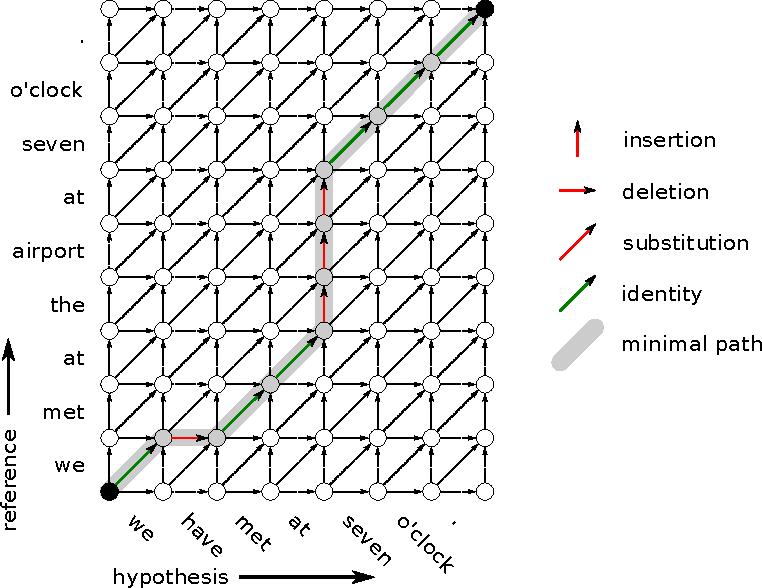
\includegraphics[width=10cm]{img/wer-grid.pdf}
    \end{center}

    \caption{An example of WER alignment grid}
    \label{wer-grid}
\end{figure}

\subsection{CDER}

The abbreviation of this metric stands for ``Cover Disjoint Error Rate'' and it
was developed by \perscite{Leusch06cder:efficient}. This metric is similar to
\metric{WER} in that it is also an edit distance based metric. In addition to the
insertions, substitutions and deletions, \metric{CDER} also allows long jumps.
The long jump is an operation in which we move in an alignment grid to any
position in the candidate (we can get to any position in an actual row of the
alignment grid for a unit price). This simulates movements of blocks (longer
sequences of tokens) and it is motivated by that block movements should not be
penalized so harshly. The \metric{CDER} is computed as follows:

\begin{equation*}
    CDER(c,r) = \frac{
        \min_{e \in E(c,r)} \left( D(e) + S(e) + I(e) + LJ(e) \right)
    }{
        |r|
    }
\end{equation*}

\noindent where $E(c,r)$ denotes a set of all sequences of edit operations
which transform the candidate $c$ to the reference $r$, and $D(e)$, $S(e)$,
$I(e)$, $LJ(e)$ denote the number of deletions, substitutions, insertions and long
jumps respectively in the sequence $s$. You can see an example of an alignment grid with
long jumps in Figure \ref{cder-grid}.

\begin{figure}
    \begin{center}
        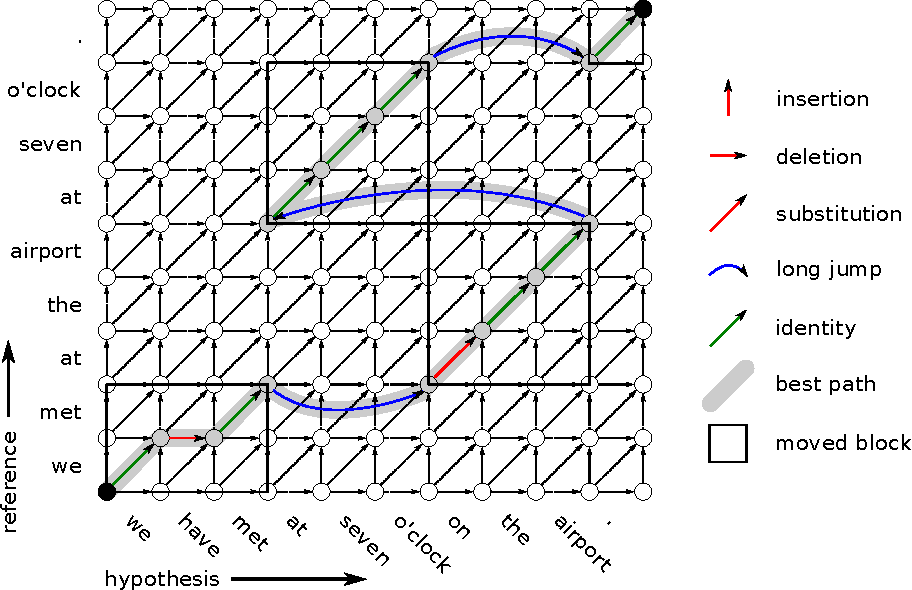
\includegraphics[width=12cm]{img/cder-grid.pdf}
    \end{center}

    \caption{An example of CDER alignment grid with long jumps}
    \label{cder-grid}
\end{figure}

\subsection{DiscoTK}

\metric{DiscoTK} metric family was developed by \perscite{wmt14-metric-discotk}.
Its abbreviation stands for ``Discourse Tree Kernel''. The basic principle is
that both reference and candidate translations are parsed to discourse parse
trees which are then compared using convolution tree kernels. There are 5
different discourse tree representations; all of them are compared and
normalized kernels scores are then averaged with uniform weights to get the
\metric{DiscoTK-light} score.  Please see the paper for more details.

One of the weaknesses of the above discourse-based metrics is that they use
unigram lexical information, which does not capture reordering. To make a more
robust metric, \perscite{wmt14-metric-discotk} combined the above five measures
with twelve more metrics implemented by \perscite{gimenez2010linguistic} in the
\textsc{Asiya} toolkit.\footnote{\url{http://nlp.lsi.upc.edu/asiya/}}. The 17
measures in total are then averaged with uniform weights to get
\metric{DiscoTK-party} score. The second variant of this metric,
\metric{DiscoTK-party-tuned}, averages the measures with tuned weights.

\subsection{LAYERED}

\metric{LAYERED} was developed by \perscite{wmt14-metric-layered}. Its name
comes from combining metrics on various linguistic layers:

\begin{itemize}

    \item \textbf{Lexical Layer.} The authors decided to use ordinary
        \metric{BLEU} from this layer.

    \item \textbf{Syntactic Layer.} \metric{LAYERED} employs three metrics
        working on this layer, 
        all of them are permutation based
        metrics and therefore consider only reordering of words. Permutations
        are constructed from source-candidate and source-reference alignments.
        The first two metrics are designed by \perscite{birch2011reordering}.

        The first metric is Hamming Score (HAMMING), which is a normalized
        Hamming distance defined as the number of disagreements between two
        permutations: $\left| \left\{ i \in \{1 \ldots n\} \mid \pi(i) \ne
        \sigma(i) \right\} \right|$. 

        The second metric is Kendall's $\tau$ distance (\metric{KTD}), which
        measures the minimum number of transpositions of two adjacent symbols
        necessary to transform one permutation into another.
        
        The last metric
        is Spearman rank correlation coefficient (\metric{SPEARMAN}), which
        measures how much the permutation between the candidate and the
        reference is monotone. (We also use Spearman rank correlation coefficient
        for the metrics evaluation. You can find the exact definition later in
        this chapter).

    \item \textbf{Semantic Layer.} There are two metrics working on this layer.
        Both of them compute precision and recall of matched dependencies in
        candidate and reference parse trees and then average them to get a
        single score.\footnote{A question is why the authors do not use
            F-measure which is usually used to combine precision and recall.
        They do not even use the terms precision and recall and instead
    define the concepts of precision and recall using a textual entailment
concept.}  The first metric (\metric{SHALLOW}) uses the Stanford dependency
parser \parcite{Marneffe06generatingtyped} to generate the dependencies. The
second metric (\metric{DEEP}) uses the UNL dependency graph generator to
construct the dependencies.

\end{itemize}

All the metrics from all the layers are then linearly combined (using tuned weights)
to get a final \metric{LAYERED} score: 

\begin{eqnarray*}
    LAYERED & = & 0.26 \cdot BLEU + 0.13 \cdot HAMMING + 0.03 \cdot KTD \\ 
            & + & 0.04 \cdot SPEARMAN + 0.28 \cdot SHALLOW + 0.26 \cdot DEEP 
\end{eqnarray*}

\subsection{Meteor}

\metric{Meteor} \parcite{wmt14-metric-meteor} evaluates candidate translations
in two phases. In the first phase, it aligns a candidate translation to a
reference translation. In the second phase, a sentence level similarity score
is computed using the constructed alignment. 

When aligning the candidate and the reference translations, the words
(sometimes phrases) in the candidate are matched to the words (phrases) in the
reference using the following matchers:

\begin{itemize}
    \item \textbf{Exact:} Matches words if their surface forms are identical.
    \item \textbf{Stem:} Matches words if their stem is identical. A language appropriate
        stemmer is used.
    \item \textbf{Synonym:} Matches words if both of them are in any synonym set according 
        to the WordNet database.
    \item \textbf{Paraphrase:} Matches phrases if they are listed in a language appropriate 
        paraphrase table. These tables can be automatically extracted from ordinary phrase tables
        used in statistical machine translation. 
\end{itemize}

Since there could be more possible alignments, the final alignment is then
resolved as the largest subset of all matches which meets the following
criteria:

\begin{enumerate}
    \item Each word in each sentence has to be covered by zero or one match.
    \item The total number of matched words in each sentence is maximal.
    \item The number of chunks is minimal (chunk is a contiguous sequence of
        candidate words which is monotonically mapped to a contiguous
        sequence of reference words).
    \item An alignment with a smaller total sum of absolute distances between
        the positions of aligned words is preferred. 
\end{enumerate}

The \metric{METEOR} for an aligned sentence is then computed as follows. Let
$h_c$ and $h_f$ be content words and function words respectively in the
hypothesis (candidate translation), and similarly let $r_c$ and $r_f$ be
content and function words in the reference. For each of the matchers $m_i$
defined above, let $m_i(h_c)$, $m_i(h_f)$ be the counts of matched content and
function words in the hypothesis and similarly let $m_i(r_c)$, $m_i(r_f)$ be
the counts of matched content and function words in the reference. Finally
a weighted precision and recall are computed:

\begin{equation*}
    P = \frac{
        \sum_i w_i \cdot ( \delta \cdot m_i(h_c) + (1-\delta) \cdot m_i(h_c))
    }{
        \delta \cdot |h_c| + (1-\delta) \cdot |h_f|
    }
\end{equation*}

\begin{equation*}
    R = \frac{
        \sum_i w_i \cdot ( \delta \cdot m_i(r_c) + (1-\delta) \cdot m_i(r_c))
    }{
        \delta \cdot |r_c| + (1-\delta) \cdot |r_f|
    }
\end{equation*}

\noindent where $w_1 \ldots w_n$ are weights of the matchers and $\delta$ is a weight
controlling the importance of content words over function words.
Using the computed precision and recall, a F mean is computed:
\begin{equation*}
    F_{mean} = \frac{
        P \cdot R
    }{
        \alpha \cdot P + (1 - \alpha) \cdot R
    }
\end{equation*}

\noindent Finally, the \metric{Meteor} score is computed as follows:

\begin{equation*}
    METEOR = (1-Pen)\cdot F_{mean}
\end{equation*}

\noindent where $Pen$ is a fragmentation penalty calculated as 

\begin{equation*}
    Pen = \gamma \cdot \left( \frac{ch}{m} \right)^\beta
\end{equation*}

\noindent where $ch$ is the number of chunks (as defined above) and $m$ is the
total number of matched words. All the parameters $\alpha$, $\beta$, $\gamma$,
$\delta$ and $w_1 \ldots w_n$ are tuned to maximize the correlation with human
judgments.

Some of the \metric{Meteor} components need language specific resources.
While some of the resources are limited to one or a few languages, other
resources can be easily trained from bilingual or monolingual data. For
example, the list of function words consists of all words with relative
frequency above a certain treshold. Paraphrase tables are constructed with a
simple method from a phrase table. The weights are tuned for each language
direction independently, however developers of \metric{Meteor} have also tuned
a universal set of weights which can be used for any language direction. This
is the case, for example, for directions from Russian and Hindi (The results
for these directions are also very poor).

%\subsection{NIST}
%\subsection{Parmesan}
%\subsection{PER}
%\subsection{RED}
%\subsection{tBLEU}
\subsection{UPC}
\subsection{VERTa}

\section{System-Level Metric Analysis}
\label{system-level}

When evaluating metrics on the system level, we would like to reward metrics
which predict the ordering of the systems as similar as possible to the
ordering given by the human scores.

While the Spearman's $\rho$ correlation coefficient was used traditionally as
the main measure of system-level metrics' quality in the past, we have decided
to use Pearson correlation coefficient as the main measure this year. We give
reasons for this change in the next subsection.

Pearson correlation coefficient is a metaevaluation metric which measures how
much two variables are linearly correlated.  In our case, the first variable is
the human score and the second variable is the metric score. We use the
following formula to compute the Pearson's $r$ for each metric and translation
direction:

\begin{equation}
    r = \frac{\sum ^n _{i=1}(H_i - \bar{H})(M_i - \bar{M})}{\sqrt{\sum ^n _{i=1}(H_i - \bar{H})^2} \sqrt{\sum ^n _{i=1}(M_i - \bar{M})^2}} 
\end{equation}

\noindent where $H$ is the vector of human scores of all the systems translating in
the given direction and $M$ is the vector of the corresponding scores as predicted
by the given metric. $\bar{H}$ and $\bar{M}$ are their means respectively.

The Pearson's $r$ ranges from -1 to 1. A value of 1 implies that a linear
equation describes the relationship between the human scores and the metric
scores and the metric score increases as the human score increases. A value of
-1 also implies a linear relationship but this time the metric score decreases
as the human score decreases. A value of 0 implies that there is no
relationship between the human scores and the metric scores.

Since we have normalized all metrics such that better translations get a higher
score, we consider metrics with values of Pearson's $r$ closer to 1 as better. 

For the sake of completeness and for the possibility to compare the results to
previous years, we also report Spearman's rank correlation coefficient in the
tables. This metaevaluation metric measures how much the human score and the
metric score are mononotonically related.  This measure does not consider the
absolute differences between the values so the relationship between the two
variables is not penalized for not being linear.  To compute Spearman's $\rho$,
we must first transform the variables to ranks.  If there are some equal
values, we assign to them an average of corresponding ranks. Once we have the
ranks, we can compute Spearman's $\rho$ as the Pearson correlation coefficient
between the rankings. Since there are no tied scores, we use the following
simplified formula: \begin{equation*} \rho = 1 - \frac{6 \sum{d_i^2}}{n(n^2
-1)} \end{equation*} where $d_i$ is the difference between the human rank and
metric's rank for system $i$ and $n$ is number of the systems. The possible
values of $\rho$ range between 1 and -1. A value of 1 implies that the metric
scores give the same ranking of the systems as the official human scores. A
value of -1 implies that the metric scores give a reversed ranking.

The reported empirical confidence intervals of system level correlations were
obtained through bootstrap resampling of 1000 samples (confidence level of
95\,\%).

\subsection{Reasons for Pearson correlation coefficient}

In the translation task, there are often similar systems with human scores very
close to each other. It can therefore easily happen that even a good metric
compares two similar systems differently from humans. We believe that the
penalty incurred by the metric for such a swap should somehow reflect that the
systems were hard to separate.

Since the Spearman's $\rho$ converts both human and metric scores to ranks and
therefore disregards the absolute differences in the scores, it does exactly what
we feel is not fair. The Pearson correlation coefficient does not suffer from this 
problem. We are aware of the fact that Pearson correlation coefficient also
reflects whether the relation between manual and automatic scores is linear (as
opposed to e.g. quadratic). We don't think this would be negatively affecting
any of the metrics since overall, the systems are of a comparable quality and
the metrics are likely to behave linearly in this small
range of scores.

\begin{figure}
    \begin{center}
        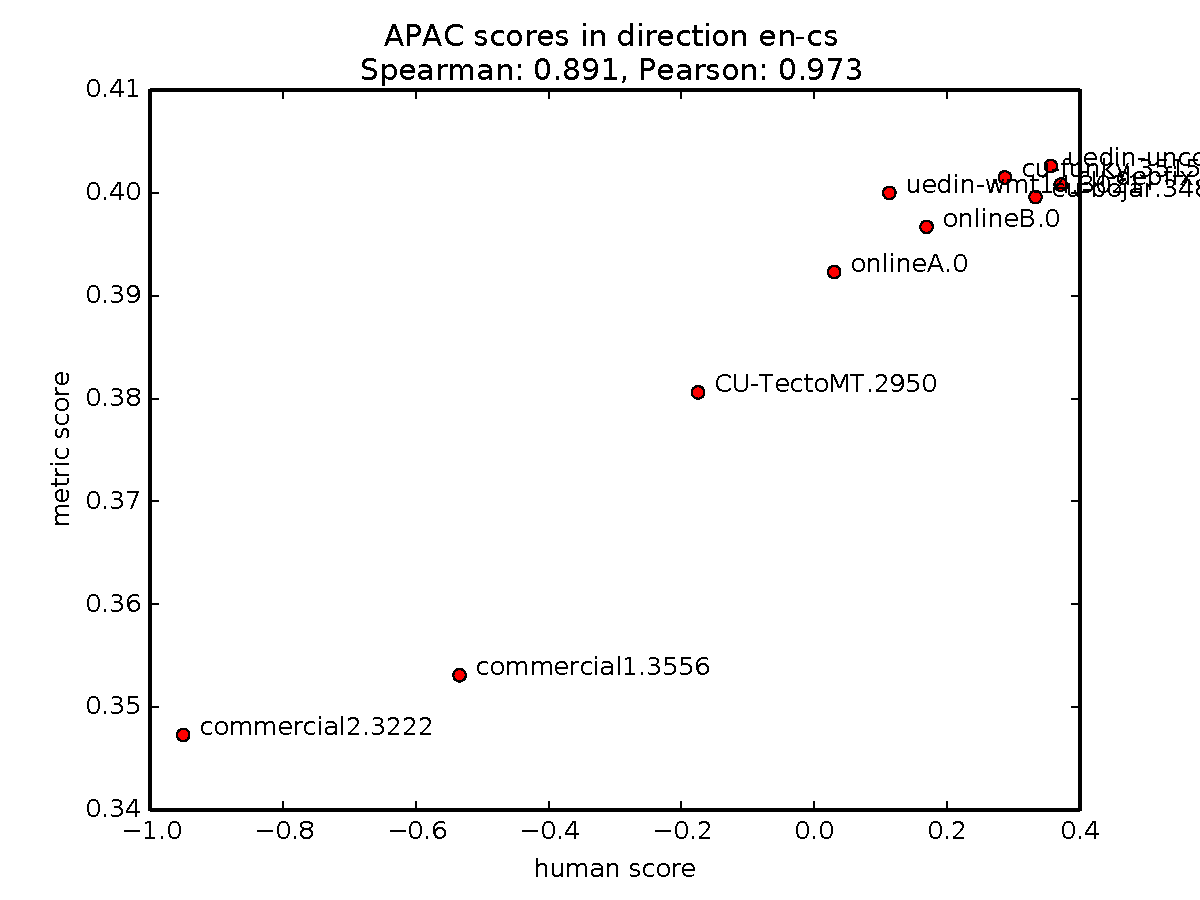
\includegraphics[width=\textwidth]{img/pearson-motivation.pdf}
    \end{center}

    \caption[Motivation for Pearson: Metric vs. human scores scatterplot]{
      Motivation for Pearson: Metric vs. human scores scatterplot
}

    \label{tree-align}
\end{figure}

You can see an example situation in Figure \ref{tree-align}. There is a cluster
of very similar systems in upper right corner. In this cluster, some systems
are not ranked correctly by a metric. For instance, the swap of the uedin-wmt14
and onlineB systems is not penalized so harshly in the Pearson score. However
in Spearman score, it is penalized just the same as a swap of very distant
systems would be penalized, for instance commercial1 and CU-TectoMT.


Moreover, the general agreement to adopt Pearson instead of Spearman's
correlation coefficient was already apparent during the WMT12 workshop. This
change just did not get through for WMT13.

\subsection{Results}

You can find the system-level correlations for translations into English in
Table \ref{system-level-corrs-toEn} and for translations out of English in
Table \ref{system-level-corrs-outEn}. Each row in the tables contains
correlations of a metric in each of the examined translation directions. The
metrics are sorted by average Pearson correlation coefficient across the
translation directions. The best results in each direction are in bold.

As in previous years, a lot of metrics outperformed \metric{BLEU} in system
level correlation. In into-English directions, metric
\metric{DiscoTK-party-tuned} has the highest correlation in two language
directions and it is also the best correlated metric on average according to both
Pearson and Spearman's coefficients. The second best correlated metric on
average (according to Pearson) is \metric{LAYERED} which is also the single
best metric in Hindi-to-English direction.  Metrics \metric{REDSys} and
\metric{REDSysSent} are quite unstable, they win in French-to-English and
Czech-to-English directions respectively but they perform very poorly in other
directions. 

Except \metric{Meteor}, none of the participants took part in the last year's
metrics task.  We can therefore compare current and last year's results only for
\metric{Meteor} and baseline metrics.  \metric{Meteor}, last year's winner,
performs generally well in some directions but it suffers horribly when
evaluating translations from non-Latin script (Russian and especially Hindi).
For the baseline metrics the results are quite similar across the years. In
both years \metric{BLEU} performs best among baseline metrics, closely followed
by \metric{CDER}. \metric{NIST} is in the middle of the list in both
years. The remaining baseline metrics \metric{TER}, \metric{WER}
and \metric{PER} perform significantly worse.

The results into German are markedly lower and have broader confidence
intervals than the results in other directions. This could be explained by a
very
high number (18) of participating systems of similar quality. 
Both human judgements and automatic metrics are negatively affected by these
circumstances. To preserve the reliability of overall metrics' performance
across languages, we
decided to exclude English-to-German
direction from the average Pearson and Spearman's correlation coefficients.

In other out-of-English directions, the best correlated metric on average according
to Pearson coefficient is \metric{NIST}, even though it does not win in any
single direction. \metric{CDER} is the second best according to Pearson
and the best metric according to Spearman's. Again it does not win in any
single direction. The metrics \metric{PER} and \metric{WER} are quite
unstable.  Each of them wins in two directions but performs very badly in
others.

Compared to the last year results, the order of metrics participating in both
years is quite similar: \metric{NIST} and \metric{CDER} performed very well
both years, followed by \metric{BLEU}. The metrics \metric{TER} and \metric{WER}
are again at the end of the list. An interesting change is that
\metric{PER} performs much better this year.


\begin{sidewaystable*}
  %\small
  \begin{center}
    \begin{tabular}{r|cccccc|c}
        \textbf{Correlation coefficient} & \multicolumn{6}{|c|}{\textbf{Pearson Correlation Coefficient}} & \textbf{Spearman's} \\
        \textbf{Direction}           & \textbf{fr-en}   & \textbf{de-en}   & \textbf{hi-en}   & \textbf{cs-en}   & \textbf{ru-en}   & \textbf{Average}   & \textbf{Average}   \\
        \textbf{Considered Systems} & 8 & 13 & 9 & 5 & 13 & \\
        \hline
        \metric{DiscoTK-party-tuned} & $.977 \pm .009$        & \best{.943 $\pm$ .020} & $.956 \pm .007$        & $.975 \pm .031$        & \best{.870 $\pm$ .022} & \best{.944 $\pm$ .018} & \best{.912 $\pm$ .043} \\
        \metric{LAYERED}             & $.973 \pm .009$        & $.893 \pm .026$        & \best{.976 $\pm$ .006} & $.941 \pm .045$        & $.854 \pm .023$        & $.927 \pm .022$        & $.894 \pm .047$        \\
        \metric{DiscoTK-party}       & $.970 \pm .010$        & $.921 \pm .024$        & $.862 \pm .015$        & $.983 \pm .025$        & $.856 \pm .023$        & $.918 \pm .019$        & $.856 \pm .046$        \\
        \metric{UPC-STOUT}           & $.968 \pm .010$        & $.915 \pm .025$        & $.898 \pm .013$        & $.948 \pm .040$        & $.837 \pm .024$        & $.913 \pm .022$        & \oosmark{$.901 \pm .045$}        \\
        \metric{VERTa-W}             & $.959 \pm .011$        & $.867 \pm .029$        & $.920 \pm .011$        & $.934 \pm .050$        & $.848 \pm .024$        & $.906 \pm .025$        & $.868 \pm .045$        \\
        \metric{VERTa-EQ}            & $.959 \pm .011$        & $.854 \pm .031$        & $.927 \pm .010$        & $.938 \pm .048$        & $.842 \pm .024$        & $.904 \pm .025$        & $.857 \pm .046$        \\
        \metric{tBLEU}               & $.952 \pm .012$        & $.832 \pm .034$        & $.954 \pm .007$        & $.957 \pm .040$        & $.803 \pm .027$        & $.900 \pm .024$        & $.841 \pm .056$        \\
        \metric{BLEU\_NRC}           & $.953 \pm .012$        & $.823 \pm .035$        & $.959 \pm .007$        & $.946 \pm .044$        & $.787 \pm .028$        & $.894 \pm .025$        & \oosmark{$.855 \pm .056$}        \\
        \metric{BLEU}                & $.952 \pm .012$        & $.832 \pm .034$        & $.956 \pm .007$        & $.909 \pm .054$        & $.789 \pm .027$        & $.888 \pm .027$        & $.833 \pm .058$        \\
        \metric{UPC-IPA}             & $.966 \pm .010$        & $.895 \pm .027$        & $.914 \pm .010$        & $.824 \pm .073$        & $.812 \pm .026$        & $.882 \pm .029$        & \oosmark{$.858 \pm .044$}        \\
        \metric{CDER}                & $.954 \pm .012$        & $.823 \pm .034$        & $.826 \pm .016$        & $.965 \pm .035$        & $.802 \pm .027$        & $.874 \pm .025$        & $.807 \pm .050$        \\
        \metric{APAC}                & $.963 \pm .010$        & $.817 \pm .034$        & $.790 \pm .016$        & $.982 \pm .026$        & $.816 \pm .026$        & $.874 \pm .022$        & $.807 \pm .049$        \\
        \metric{REDSys}              & \best{.981 $\pm$ .008} & $.898 \pm .026$        & $.676 \pm .022$        & $.989 \pm .021$        & $.814 \pm .026$        & $.872 \pm .021$        & $.786 \pm .047$        \\
        \metric{REDSysSent}          & $.980 \pm .008$        & $.910 \pm .024$        & $.644 \pm .023$        & \best{.993 $\pm$ .018} & $.807 \pm .027$        & $.867 \pm .020$        & $.771 \pm .043$        \\
        \metric{NIST}                & $.955 \pm .011$        & $.811 \pm .035$        & $.784 \pm .016$        & $.983 \pm .025$        & $.800 \pm .027$        & $.867 \pm .023$        & \oosmark{$.824 \pm .055$}        \\
        \metric{DiscoTK-light}       & $.965 \pm .011$        & $.935 \pm .022$        & $.557 \pm .025$        & $.954 \pm .038$        & $.791 \pm .027$        & $.840 \pm .024$        & $.774 \pm .046$        \\
        \metric{Meteor}              & $.975 \pm .009$        & $.927 \pm .022$        & $.457 \pm .027$        & $.980 \pm .029$        & $.805 \pm .026$        & $.829 \pm .023$        & \oosmark{$.788 \pm .046$}        \\
        \metric{TER}                 & $.952 \pm .012$        & $.775 \pm .038$        & $.618 \pm .021$        & $.976 \pm .031$        & $.809 \pm .027$        & $.826 \pm .026$        & $.746 \pm .057$        \\
        \metric{WER}                 & $.952 \pm .012$        & $.762 \pm .038$        & $.610 \pm .021$        & $.974 \pm .033$        & $.809 \pm .027$        & $.821 \pm .026$        & $.736 \pm .058$        \\
        \metric{AMBER}               & $.948 \pm .012$        & $.910 \pm .026$        & $.506 \pm .026$        & $.744 \pm .095$        & $.797 \pm .027$        & $.781 \pm .037$        & $.728 \pm .051$        \\
        \metric{PER}                 & $.946 \pm .013$        & $.867 \pm .031$        & $.411 \pm .025$        & $.883 \pm .063$        & $.799 \pm .028$        & $.781 \pm .032$        & $.698 \pm .047$        \\
        \metric{ELEXR}               & $.971 \pm .009$        & $.857 \pm .031$        & $.535 \pm .026$        & $.945 \pm .044$        & $-.404 \pm .045$       & $.581 \pm .031$        & $.652 \pm .046$        \\
        \hline
    \end{tabular}
  \end{center}
  
  \caption[System-level correlations when translating into English]{
      System-level correlations of automatic evaluation metrics and the
      official WMT human scores when translating into English.  The symbol
      ``$\wr$'' indicates where the Spearman's $\rho$ average is out of
      sequence compared to the main Pearson average.}

  \label{system-level-corrs-toEn}

\end{sidewaystable*}

\begin{sidewaystable*}[t]
  %\small

  \begin{center}
    \begin{tabular}{r|ccccc|c|c}
        \textbf{Correlation coefficient}        & \multicolumn{6}{|c|}{\textbf{Pearson Correlation Coefficient}} & \textbf{Spearman's} \\
        \textbf{Direction} & \textbf{en-fr} & \textbf{en-hi} & \textbf{en-cs} & \textbf{en-ru} & \textbf{Average} & \textbf{en-de} & \textbf{Average} \\
        \textbf{Considered Systems} & 13 & 12 & 10 & 9 & & 18 & (excl. en-de)\\
        \hline
        \metric{NIST}       & $.941 \pm .022$        & $.981 \pm .006$        & $.985 \pm .006$        & $.927 \pm .012$        & \best{.959 $\pm$ .012} & $.200 \pm .046$        & \best{.850 $\pm$ .030} \\
        \metric{CDER}       & $.949 \pm .020$        & $.949 \pm .010$        & $.982 \pm .006$        & $.938 \pm .011$        & $.955 \pm .012$        & $.278 \pm .045$        & $.840 \pm .036$        \\
        \metric{AMBER}      & $.928 \pm .023$        & \best{.990 $\pm$ .004} & $.972 \pm .008$        & $.926 \pm .012$        & $.954 \pm .012$        & $.241 \pm .045$        & $.817 \pm .041$        \\
        \metric{Meteor}     & $.941 \pm .021$        & $.975 \pm .007$        & $.976 \pm .007$        & $.923 \pm .013$        & $.954 \pm .012$        & $.263 \pm .045$        & $.806 \pm .039$        \\
        \metric{BLEU}       & $.937 \pm .022$        & $.973 \pm .007$        & $.976 \pm .007$        & $.915 \pm .013$        & $.950 \pm .012$        & $.216 \pm .046$        & \oosmark{$.809 \pm .036$}        \\
        \metric{PER}        & $.936 \pm .023$        & $.931 \pm .011$        & \best{.988 $\pm$ .005} & \best{.941 $\pm$ .011} & $.949 \pm .013$        & $.190 \pm .047$        & \oosmark{$.823 \pm .037$}        \\
        \metric{APAC}       & $.950 \pm .020$        & $.940 \pm .011$        & $.973 \pm .008$        & $.929 \pm .012$        & $.948 \pm .013$        & $.346 \pm .044$        & $.799 \pm .041$        \\
        \metric{tBLEU}      & $.932 \pm .023$        & $.968 \pm .008$        & $.973 \pm .008$        & $.912 \pm .013$        & $.946 \pm .013$        & $.239 \pm .046$        & \oosmark{$.805 \pm .039$}        \\
        \metric{BLEU\_NRC}  & $.933 \pm .022$        & $.971 \pm .007$        & $.974 \pm .008$        & $.901 \pm .014$        & $.945 \pm .013$        & $.205 \pm .046$        & \oosmark{$.809 \pm .039$}        \\
        \metric{ELEXR}      & $.885 \pm .029$        & $.962 \pm .009$        & $.979 \pm .007$        & $.938 \pm .011$        & $.941 \pm .014$        & $.260 \pm .044$        & $.768 \pm .036$        \\
        \metric{TER}        & $.954 \pm .019$        & $.829 \pm .017$        & $.978 \pm .007$        & $.931 \pm .012$        & $.923 \pm .014$        & $.324 \pm .045$        & $.745 \pm .035$        \\
        \metric{WER}        & \best{.960 $\pm$ .018} & $.516 \pm .026$        & $.976 \pm .007$        & $.932 \pm .011$        & $.846 \pm .016$        & \best{.357 $\pm$ .045} & $.696 \pm .037$        \\
        \hline
        \metric{Parmesan}   & n/a                      & n/a                      & $.962 \pm .009$        & n/a                      & $.962 \pm .009$        & n/a                      & $.915 \pm .048$        \\
        \metric{UPC-IPA}    & $.940 \pm .021$        & n/a                      & $.969 \pm .008$        & $.921 \pm .013$        & $.943 \pm .014$        & $.285 \pm .045$        & $.785 \pm .050$        \\
        \metric{REDSysSent} & $.941 \pm .021$        & n/a                      & n/a                      & n/a                      & $.941 \pm .021$        & $.208 \pm .045$        & \oosmark{$.962 \pm .038$}        \\
        \metric{REDSys}     & $.940 \pm .021$        & n/a                      & n/a                      & n/a                      & $.940 \pm .021$        & $.208 \pm .045$        & $.962 \pm .038$        \\
        \metric{UPC-STOUT}  & $.940 \pm .021$        & n/a                      & $.938 \pm .011$        & $.919 \pm .013$        & $.933 \pm .015$        & $.301 \pm .044$        & $.713 \pm .040$        \\
        \hline
    \end{tabular}
  \end{center}

  \caption[System-level correlations when translating out of
  English]{System-level correlations of automatic evaluation metrics and the
      official WMT human scores when translating out of English.  The symbol
      ``$\wr$'' indicates where the Spearman's $\rho$ average is out of
      sequence compared to the main Pearson average.}

  \label{system-level-corrs-outEn}
\end{sidewaystable*}
\afterpage{\clearpage}

\section{Segment-Level Metric Analysis}
\label{segment-level}

We measure the quality of metrics' segment-level scores using Kendall's $\tau$
rank correlation coefficient. In this type of evaluation, a metric is expected
to predict the result of the manual pairwise comparison of two systems. Note
that the golden truth is obtained from a compact annotation of five systems at
once, while an experiment with text-to-speech evaluation techniques by
\perscite{vazquez-alvarez-huckvale:2002} suggests that a genuine pairwise
comparison is likely to lead to more stable results.

In the past, slightly different variations of
Kendall's $\tau$ computation were used in the Metrics Tasks. Also some of the
participants have noticed a problem with ties in the WMT13 method. Therefore, we
discuss several possible variants in detail in this paper.

\subsection{Notation for Kendall's $\tau{}$ computation}

The basic formula for Kendall's $\tau$ is:

\begin{equation}
    \tau = \frac{|Concordant| - |Discordant|}{|Concordant| + |Discordant|}
\end{equation}

\noindent where $Concordant$ is the set of all human comparisons for which a
given metric suggests the same order and $Discordant$ is the set of all human comparisons for
which a given metric disagrees.
For an example of Kendall's $\tau$ computation, let us have the following comparisons:
\begin{center}
\begin{tabular}{cc}
  Human & Metric \\
  \hline
  $A < B$ & $A < B$ \\
  $C > A$ & $C > A$ \\
  $C > B$ & $C < B$ \\
\end{tabular}
\end{center}

\noindent There are two concordant comparisons and one discordant:

\begin{equation*}
  \tau = \frac{2-1}{2+1} = \frac{1}{3}
\end{equation*}

In the original Kendall's $\tau$, comparisons
with human or metric ties are considered neither concordant nor discordant.
However in the previous Metrics Tasks (\cite{callisonburch:wmt12} and
earlier), comparisons with human ties were considered as discordant.
To easily specify which pairs are counted as concordant and which as discordant, we
have developed the following tabular notation. This is, for example, the WMT12
method:

\begin{center}
  \begin{tabular}{cc|ccc}
                                             &     & \multicolumn{3}{c}{Metric} \\  
                  \multicolumn{2}{c|}{WMT12}       & $<$ & $=$ & $>$ \\ \hline
      \multirow{3}{*}{\rotatebox{90}{Human}} & $<$ &  1  & -1  & -1  \\
                                             & $=$ &  X  &  X  &  X  \\ 
                                             & $>$ & -1  & -1  &  1  \\ 
  \end{tabular}
\end{center}

% \noindent
Given such a matrix $C_{h,m}$ where $h,m \in \{<,=,>\}$\footnote{Here
the relation $<$ always means ``is better than'' even for metrics
where the better system receives a higher score.} and a metric we compute the
Kendall's $\tau$ the following way:
We insert each extracted human pairwise comparison into exactly one of the nine
sets $S_{h,m}$ according to human and metric ranks. For example the set
$S_{<,>}$ contains all comparisons where the left-hand system was ranked better
than right-hand system by humans and it was ranked the other way round by the
metric in question.
To compute the numerator of Kendall's $\tau$, we take the coefficients from the matrix
$C_{h,m}$, use them to multiply the sizes of the corresponding sets $S_{h,m}$ and
then sum them up. We do not include sets for which the value of $C_{h,m}$ is X.
To compute the denominator of Kendall's $\tau$, we simply sum the sizes of all
the sets
$S_{h,m}$ except those where $C_{h,m} = \text{X}$. To define it formally:

\begin{equation*}
    \tau = \frac{
        \sum\limits_{\substack{
            h,m \in \{<,=,>\} \\
            C_{h,m} \ne \text{X}
        }}
        C_{h,m} |S_{h,m}|
    }{
        \sum\limits_{\substack{
            h,m \in \{<,=,>\} \\
            C_{h,m} \ne \text{X}
        }}
        |S_{h,m}|
    }
\end{equation*}

For an example of WMT12 computation, let us have the following comparisons:
\begin{center}
\begin{tabular}{cc}
  Human & Metric \\
  \hline
  $A < B$ & $A < B$ \\
  $A < B$ & $A < B$ \\
  $A > B$ & $A = B$ \\
  $A = B$ & $A > B$ \\
\end{tabular}
\end{center}

\noindent The Kendall's $\tau$ score is then computed in the following way:

\begin{equation*}
  \tau = \frac{2-1}{2+1} = \frac{1}{3}
\end{equation*}

\subsection{Discussion on Kendall's $\tau{}$ computation}

In 2013, we thought that metric ties should not be penalized and we decided to
excluded them like the human ties. We will denote this method as WMT13:

\begin{center}
  \begin{tabular}{cc|ccc}
                                             &     & \multicolumn{3}{c}{Metric} \\  
                  \multicolumn{2}{c|}{WMT13}       & $<$ & $=$ & $>$ \\ \hline
      \multirow{3}{*}{\rotatebox{90}{Human}} & $<$ &  1  &  X  & -1  \\
                                             & $=$ &  X  &  X  &  X  \\ 
                                             & $>$ & -1  &  X  &  1  \\ 
  \end{tabular}
\end{center}

\noindent It turned out, however, that it was not a good idea: metrics could
game the scoring by avoiding hard cases and assigning lots of ties. A natural
solution is to count the metrics ties also in the denominator to avoid the problem.
We will denote this variant as WMT14:

\begin{center}
  \begin{tabular}{cc|ccc}
                                             &     & \multicolumn{3}{c}{Metric} \\  
                  \multicolumn{2}{c|}{WMT14}       & $<$ & $=$ & $>$ \\ \hline
      \multirow{3}{*}{\rotatebox{90}{Human}} & $<$ &  1  &  0  & -1  \\
                                             & $=$ &  X  &  X  &  X  \\ 
                                             & $>$ & -1  &  0  &  1  \\ 
  \end{tabular}
\end{center}

\noindent The WMT14 variant does not allow for gaming the scoring like the WMT13
variant does. Compared to WMT12 method, WMT14 does not penalize ties.

%has the following advantage: In WMT12
%a metric could intentionally randomly pertrubate the scores to avoid the tied
%scores. In half of the originally tied cases it would get into   moved tied comparisons from
%discordant pairs to concordant. 

We also considered getting human ties involved. The most natural variant would be the
following variant denoted as HTIES:

\begin{center}
  \begin{tabular}{cc|ccc}
                                             &     & \multicolumn{3}{c}{Metric} \\  
    \multicolumn{2}{c|}{HTIES}                  & $<$ & $=$ & $>$ \\ \hline
      \multirow{3}{*}{\rotatebox{90}{Human}} & $<$ &  1  &  0  & -1  \\
                                             & $=$ &  0  &  1  &  0  \\ 
                                             & $>$ & -1  &  0  &  1  \\ 
  \end{tabular}
\end{center}

\noindent Unfortunately this method allows for gaming the scoring as well. The
least risky choice for metrics in hard cases would be to assign a tie because
it cannot worsen the Kendall's $\tau$ and there is quite a high chance that the
human rank is also a tie.  Metrics could be therefore tuned to predict ties
often but such metrics are not very useful. For example, the simplistic metric
which assigns the same score to all candidates (and therefore all pairs would
be tied by the metric) would get the score equal to the proportion of ties in
all human comparisons.  It would become one of the best performing metrics in
WMT13 even though it is not informative at all.

We have decided to use WMT14 variant as the main evaluation measure this year,
however, we are also reporting average scores computed by other variants.


\subsection{Kendall's $\tau$ results}

\begin{sidewaystable*}[t]
  \begin{center}
    %\tiny
    \begin{tabular}{r|cccccc}
        \textbf{Direction}           & \textbf{fr-en}           & \textbf{de-en}           & \textbf{hi-en}           & \textbf{cs-en}           & \textbf{ru-en}           & \textbf{Avg} \\
        \textbf{Extracted-pairs}     & 26090                    & 25260                    & 20900                    & 21130                    & 34460                    &              \\
        \hline
        \metric{DiscoTK-party-tuned} & \best{.433 $\pm$ .012} & \best{.380 $\pm$ .013} & $.434 \pm .013$        & \best{.328 $\pm$ .015} & \best{.355 $\pm$ .011} & \best{.386 $\pm$ .013} \\
        \metric{BEER}                & $.417 \pm .013$        & $.337 \pm .014$        & \best{.438 $\pm$ .013} & $.284 \pm .016$        & $.333 \pm .011$        & $.362 \pm .013$        \\
        \metric{REDcombSent}         & $.406 \pm .012$        & $.338 \pm .014$        & $.417 \pm .013$        & $.284 \pm .015$        & $.336 \pm .011$        & $.356 \pm .013$        \\
        \metric{REDcombSysSent}      & $.408 \pm .012$        & $.338 \pm .014$        & $.416 \pm .013$        & $.282 \pm .014$        & $.336 \pm .011$        & $.356 \pm .013$        \\
        \metric{Meteor}              & $.406 \pm .012$        & $.334 \pm .014$        & $.420 \pm .013$        & $.282 \pm .015$        & $.329 \pm .010$        & $.354 \pm .013$        \\
        \metric{REDSysSent}          & $.404 \pm .012$        & $.338 \pm .014$        & $.386 \pm .014$        & $.283 \pm .015$        & $.321 \pm .010$        & $.346 \pm .013$        \\
        \metric{REDSent}             & $.403 \pm .012$        & $.336 \pm .014$        & $.383 \pm .014$        & $.283 \pm .015$        & $.323 \pm .011$        & $.345 \pm .013$        \\
        \metric{UPC-IPA}             & $.412 \pm .012$        & $.340 \pm .014$        & $.368 \pm .014$        & $.274 \pm .015$        & $.316 \pm .011$        & $.342 \pm .013$        \\
        \metric{UPC-STOUT}           & $.403 \pm .012$        & $.345 \pm .014$        & $.352 \pm .014$        & $.275 \pm .015$        & $.317 \pm .011$        & $.338 \pm .013$        \\
        \metric{VERTa-W}             & $.399 \pm .013$        & $.321 \pm .015$        & $.386 \pm .014$        & $.263 \pm .015$        & $.315 \pm .011$        & $.337 \pm .014$        \\
        \metric{VERTa-EQ}            & $.407 \pm .013$        & $.315 \pm .014$        & $.384 \pm .013$        & $.263 \pm .015$        & $.312 \pm .011$        & $.336 \pm .013$        \\
        \metric{DiscoTK-party}       & $.395 \pm .013$        & $.334 \pm .014$        & $.362 \pm .013$        & $.264 \pm .016$        & $.305 \pm .011$        & $.332 \pm .013$        \\
        \metric{AMBER}               & $.367 \pm .013$        & $.313 \pm .014$        & $.362 \pm .013$        & $.246 \pm .016$        & $.294 \pm .011$        & $.316 \pm .013$        \\
        \metric{BLEU\_NRC}           & $.382 \pm .013$        & $.272 \pm .014$        & $.322 \pm .014$        & $.226 \pm .016$        & $.269 \pm .011$        & $.294 \pm .013$        \\
        \metric{sentBLEU}            & $.378 \pm .013$        & $.271 \pm .014$        & $.300 \pm .013$        & $.213 \pm .016$        & $.263 \pm .011$        & $.285 \pm .013$        \\
        \metric{APAC}                & $.364 \pm .012$        & $.271 \pm .014$        & $.288 \pm .014$        & $.198 \pm .016$        & $.276 \pm .011$        & $.279 \pm .013$        \\
        \metric{DiscoTK-light}       & $.311 \pm .014$        & $.224 \pm .015$        & $.238 \pm .013$        & $.187 \pm .016$        & $.209 \pm .011$        & $.234 \pm .014$        \\
        \metric{DiscoTK-light-kool}  & $.005 \pm .001$        & $.001 \pm .000$        & $.000 \pm .000$        & $.002 \pm .001$        & $.001 \pm .000$        & $.002 \pm .001$        \\
        \hline
    \end{tabular}
  \end{center}

  \caption[Segment-level correlations when translating into
  English]{Segment-level Kendall's $\tau$ correlations of automatic evaluation
      metrics and the official WMT human judgements when translating into
      English.
  }

  \label{segment-level-correlations-toEn}
\end{sidewaystable*}


\begin{sidewaystable*}[t]
  \begin{center}
    %\tiny
    \begin{tabular}{r|cccccc}
        \textbf{Direction}      & \textbf{en-fr}           & \textbf{en-de}           & \textbf{en-hi}           & \textbf{en-cs}           & \textbf{en-ru}           & \textbf{Avg} \\
        \textbf{Extracted-pairs}& 33350                    & 54660                    & 28120                    & 55900                    & 28960                    &              \\
        \hline
        \metric{BEER}           & $.292 \pm .012$        & \best{.268 $\pm$ .009} & $.250 \pm .013$        & \best{.344 $\pm$ .009} & \best{.440 $\pm$ .013} & \best{.319 $\pm$ .011} \\
        \metric{Meteor}         & $.280 \pm .012$        & $.238 \pm .009$        & $.264 \pm .012$        & $.318 \pm .009$        & $.427 \pm .012$        & $.306 \pm .011$        \\
        \metric{AMBER}          & $.264 \pm .012$        & $.227 \pm .009$        & \best{.286 $\pm$ .012} & $.302 \pm .009$        & $.397 \pm .013$        & $.295 \pm .011$        \\
        \metric{BLEU\_NRC}      & $.261 \pm .012$        & $.202 \pm .009$        & $.234 \pm .013$        & $.297 \pm .009$        & $.391 \pm .012$        & $.277 \pm .011$        \\
        \metric{APAC}           & $.253 \pm .012$        & $.210 \pm .008$        & $.203 \pm .012$        & $.292 \pm .009$        & $.388 \pm .013$        & $.269 \pm .011$        \\
        \metric{sentBLEU}       & $.256 \pm .012$        & $.191 \pm .009$        & $.227 \pm .012$        & $.290 \pm .009$        & $.381 \pm .013$        & $.269 \pm .011$        \\
        \hline
        \metric{UPC-STOUT}      & $.279 \pm .011$        & $.234 \pm .008$        & n/a                      & $.282 \pm .009$        & $.425 \pm .013$        & $.305 \pm .011$      \\
        \metric{UPC-IPA}        & $.264 \pm .012$        & $.227 \pm .009$        & n/a                      & $.298 \pm .009$        & $.426 \pm .013$        & $.304 \pm .011$      \\
        \metric{REDSent}        & \best{.293 $\pm$ .012} & $.242 \pm .009$        & n/a                      & n/a                      & n/a                      & $.267 \pm .010$  \\
        \metric{REDcombSysSent} & $.291 \pm .012$        & $.244 \pm .009$        & n/a                      & n/a                      & n/a                      & $.267 \pm .010$  \\
        \metric{REDcombSent}    & $.290 \pm .012$        & $.242 \pm .009$        & n/a                      & n/a                      & n/a                      & $.266 \pm .010$  \\
        \metric{REDSysSent}     & $.290 \pm .012$        & $.239 \pm .008$        & n/a                      & n/a                      & n/a                      & $.264 \pm .010$  \\
        \hline
    \end{tabular}
  \end{center}

  \caption[Segment-level correlations when translating out of
  English]{Segment-level Kendall's $\tau$ correlations of automatic evaluation
      metrics and the official WMT human judgements when translating out of
      English.
 }

  \label{segment-level-correlations-fromEn}
\end{sidewaystable*}

\begin{table}[t]
  \begin{center}
    \small
    \begin{tabular}{r|cccc}
      \textbf{Metric}              & \textbf{WMT14}           & \textbf{WMT12}           & \textbf{WMT13}           & \textbf{HTIES}           \\
        \hline
        \metric{DiscoTK-party-tuned} & \best{.386 $\pm$ .013} & \best{.386 $\pm$ .013} & $.386 \pm .013$        & $.306 \pm .010$        \\
        \metric{BEER}                & $.362 \pm .013$        & $.358 \pm .013$        & $.363 \pm .013$        & \oosmark{\best{.318 $\pm$ .011}} \\
        \metric{REDcombSent}         & $.356 \pm .013$        & $.346 \pm .013$        & $.360 \pm .013$        & $.317 \pm .011$        \\
        \metric{REDcombSysSent}      & $.356 \pm .013$        & $.346 \pm .013$        & $.359 \pm .013$        & $.316 \pm .010$        \\
        \metric{Meteor}              & $.354 \pm .013$        & $.341 \pm .013$        & $.359 \pm .013$        & \oosmark{$.317 \pm .010$}        \\
        \metric{REDSysSent}          & $.346 \pm .013$        & $.335 \pm .013$        & $.350 \pm .013$        & $.309 \pm .010$        \\
        \metric{REDSent}             & $.345 \pm .013$        & $.334 \pm .013$        & $.349 \pm .013$        & $.308 \pm .010$        \\
        \metric{UPC-IPA}             & $.342 \pm .013$        & \oosmark{$.340 \pm .014$}        & $.343 \pm .014$        & $.300 \pm .011$        \\
        \metric{UPC-STOUT}           & $.338 \pm .013$        & $.336 \pm .013$        & $.339 \pm .013$        & $.294 \pm .011$        \\
        \metric{VERTa-W}             & $.337 \pm .014$        & $.320 \pm .014$        & \oosmark{$.342 \pm .014$}        & \oosmark{$.304 \pm .011$}        \\
        \metric{VERTa-EQ}            & $.336 \pm .013$        & \oosmark{$.323 \pm .013$}        & $.341 \pm .013$        & $.302 \pm .011$        \\
        \metric{DiscoTK-party}       & $.332 \pm .013$        & \oosmark{$.332 \pm .013$}        & $.332 \pm .013$        & $.263 \pm .011$        \\
        \metric{AMBER}               & $.316 \pm .013$        & $.302 \pm .013$        & $.321 \pm .014$        & \oosmark{$.286 \pm .011$}        \\
        \metric{BLEU\_NRC}           & $.294 \pm .013$        & $.267 \pm .014$        & $.303 \pm .014$        & $.271 \pm .011$        \\
        \metric{sentBLEU}            & $.285 \pm .013$        & $.258 \pm .014$        & $.293 \pm .014$        & $.264 \pm .011$        \\
        \metric{APAC}                & $.279 \pm .013$        & $.243 \pm .014$        & $.290 \pm .014$        & $.261 \pm .011$        \\
        \metric{DiscoTK-light}       & $.234 \pm .014$        & $.234 \pm .014$        & $.234 \pm .014$        & $.184 \pm .011$        \\
        \metric{DiscoTK-light-kool}  & $.002 \pm .001$        & $-.996 \pm .001$       & \oosmark{\best{.676 $\pm$ .256}} & \oosmark{$.211 \pm .005$}        \\
        \hline
    \end{tabular}
  \end{center}

  
  \caption[Averages of other variants of Kendall's $\tau$ in directions into English ] { This table
    contains average segment-level Kendall's $\tau$ computed by other variants
    in directions into English. The average correlation of WMT14 variant is
    repeated in the first column. The symbol ``$\wr$'' indicates where the
  averages of other variants are out of sequence compared to the WMT14
variant.}

  \label{kendall-other-variants-toEn}
\end{table}


\begin{table}[t]
  \begin{center}
    \small
    \begin{tabular}{r|cccc}
      \textbf{Metric}          & \textbf{WMT14}                         & \textbf{WMT12}           & \textbf{WMT13}           & \textbf{HTIES}           \\
        \hline
        \metric{BEER}           & \best{.319 $\pm$ .011} & \best{.314 $\pm$ .011} & \best{.320 $\pm$ .011} & $.272 \pm .009$        \\
        \metric{Meteor}         & $.306 \pm .011$        & $.283 \pm .011$        & $.313 \pm .011$        & \oosmark{\best{.273 $\pm$ .008}} \\
        \metric{AMBER}          & $.295 \pm .011$        & $.269 \pm .011$        & $.303 \pm .011$        & $.266 \pm .009$        \\
        \metric{BLEU\_NRC}      & $.277 \pm .011$        & $.235 \pm .011$        & $.289 \pm .011$        & $.256 \pm .009$        \\
        \metric{APAC}           & $.269 \pm .011$        & $.217 \pm .011$        & $.285 \pm .011$        & $.252 \pm .008$        \\
        \metric{sentBLEU}       & $.269 \pm .011$        & \oosmark{$.232 \pm .011$}        & $.280 \pm .011$        & $.246 \pm .009$        \\
        \hline
        \metric{UPC-STOUT}        & $.305 \pm .011$        & $.300 \pm .010$        & $.306 \pm .011$        & $.256 \pm .008$        \\
        \metric{UPC-IPA}          & $.304 \pm .011$        & $.292 \pm .011$        & \oosmark{$.308 \pm .011$}        & \oosmark{$.259 \pm .008$}        \\
        \metric{REDSent}              & $.267 \pm .010$        & $.246 \pm .010$        & $.273 \pm .011$        & $.257 \pm .008$        \\
        \metric{REDcombSysSent}       & $.267 \pm .010$        & \oosmark{$.249 \pm .010$}        & $.272 \pm .010$        & $.256 \pm .008$        \\
        \metric{REDcombSent}          & $.266 \pm .010$        & $.248 \pm .010$        & $.271 \pm .011$        & $.256 \pm .008$        \\
        \metric{REDSysSent}           & $.264 \pm .010$        & $.235 \pm .010$        & \oosmark{$.273 \pm .010$}        & \oosmark{$.257 \pm .008$}        \\
        \hline
    \end{tabular}
  \end{center}

  \caption[Averages of other variants of Kendall's $\tau$ in directions out of English] { This table
    contains average segment-level Kendall's $\tau$ computed by other variants
    in directions out of English. The average correlation of WMT14 variant is
    repeated in the first column. The symbol ``$\wr$'' indicates where the
  averages of other variants are out of sequence compared to the WMT14
variant.}

  \label{kendall-other-variants-fromEn}
\end{table}

\afterpage{\clearpage}




The final Kendall's $\tau$ results are shown in Table
\ref{segment-level-correlations-toEn} for directions into English and in Table
\ref{segment-level-correlations-fromEn} for directions out of English.  Each
row in the tables contains correlations of a metric in given directions. The
metrics are sorted by the average correlation across translation directions.  The
highest correlation in each column is in bold. Table
\ref{kendall-other-variants-toEn} and Table \ref{kendall-other-variants-fromEn}
contain average Kendall's $\tau$ computed by other variants including the
variant WMT13 used last year.  Metrics which did not compute scores in all
directions are at the bottom of the tables. The possible values of $\tau$ range
between -1 (a metric always predicted a different order than humans did) and 1
(a metric always predicted the same order as humans did). Metrics with a higher
$\tau$ are better.

We also computed empirical confidence intervals of Kendall's $\tau$ using bootstrap
resampling. We varied the ``golden truth'' by sampling from human judgments. We
have generated 1000 new sets and report the average of the upper and lower
2.5\,\% empirical bound, which corresponds to the 95\,\% confidence interval.
%XXX Matousi, je tenhle popis srozumitelny?




In directions into English (Table~\ref{segment-level-correlations-toEn}), the
strongest correlated segment-level metric on average is
\metric{DiscoTK-party-tuned} followed by \metric{BEER}. Unlike the system level
correlation, the results are much more stable here.
\metric{DiscoTK-party-tuned} has the highest correlation in 4 of 5 language
directions. Generally, the ranking of metrics is almost the same in each
direction. 

The only two metrics which also participated in last year metrics task are
\metric{Meteor} and \metric{sentBLEU}. In both years, \metric{Meteor} performed
quite well unlike \metric{sentBLEU} which was outperformed by most of the
metrics. 

The metric \metric{DiscoTK-light-kool} is worth mentioning.  It is deliberately
designed to assign the same score for all systems for most of the segments.  It
obtained scores very close to zero (i.e. totally uninformative) in the WMT14
variant.  In WMT13 thought, it reached the highest score.

In directions out of English (Table~\ref{segment-level-correlations-fromEn}),
the metric with highest correlation on average across all directions is
\metric{Beer}, followed by \metric{Meteor}.

\section{Overall Comparison of Automatic Metrics}

\XXX{Tady tu sekci se teprve chystam predelat}

In this paper, we summarized the results of the WMT14 Metrics Shared Task, which
assesses the quality of
various automatic machine translation metrics. As in previous years, human
judgements collected in WMT14 serve as the golden truth and we check how well
the metrics predict the judgements at the level of individual sentences as well
as at the level of the whole test set (system-level).

This year, neither the system-level nor the segment-level scores are directly
comparable to the previous years. The system-level scores are affected by the
change of the underlying interpretation of the collected judgements in the main
translation task evaluation as well as
our choice of Pearson coefficient instead of Spearman's rank correlation. The
segment-level scores are affected by the different handling of ties this year.
Despite somewhat sacrificing the year-to-year comparability, we believe all
changes are towards a fairer evaluation and thus better in the long term.

As in previous years, segment-level correlations are much lower than
system-level ones, reaching at most Kendall's $\tau$ of 0.45 for the best
performing metric in the best language pair. So, there is quite some research
work to be done. We are happy to see that many new metrics emerged this year,
which also underlines the importance of the Metrics Shared Task.



\chapter{Implementation Details}
\XXX{Nevim, jak moc podrobne. Hlavne popsat annotacni aplikace, datovy model,
pouzite frameworky a knihovny. Strucne popsat implementaci ostatnich skriptu,
co ktery dela.}

\chapter{Conclusion}
\label{chapter:conclusion}

\section{Manual and Semiautomatic Evaluation}

In this thesis, we proposed a new method for manual evaluation, called
\metoda{SegRanks}, in which annotators rank short segments (up to six words) of
a translated sentence relatively to each other. The ranking of short segments
is easier for annotators, since the they do not have to read and remember whole
sentences at once. The most promising benefit of this method is that short
segments are often translated identically.  We can take advantage of this in
two ways: First, annotators are shown identical segments only once so that they
do not have to rank them multiple times. Second, the evaluated segments can be
stored together with their ranks in a database, which can be used later to
automatically evaluate unseen sentences or to tune a system's parameters. We
also discussed disadvantages of this method. The most severe ones are that the
extracted segments do not always cover the whole sentence and that the segments
are evaluated without their sentence context.

We developed an easy-to-use and modern annotation interface and conducted a
manual evaluation experiment using the proposed method. We evaluated the
systems which participated in the English-Czech direction in WMT Translation
Task. The measured the inter- and intra-annotator $\kappa$ scores (the
normalized agreement) are higher than the corresponding values in the WMT
manual evaluation, which means that our evaluation method is more robust.

To get a final score for each system's translation, we compute how often the
segments of the system were ranked better than other segments (in the context
of pairwise comparisons).  The results of evaluated systems are quite similar
to the results obtained by the official WMT judgments. However, our method is
not able to correctly distinguish some systems with very similar quality. The
Pearson correlation coefficient between the \metoda{SegRanks} scores and the
official human scores is 0.978, which is lower than correlation of some of the
best performing automatic metrics (\metric{NIST}, \metric{CDER},
\metric{ELEXR}). We manually analyzed sentences which were ranked high in the
short segment judgments but ranked low in the official WMT judgment to explain
the difference. In most of these sentences, there was a badly translated part
which was, however, not covered with evaluated short segments.  The uncovered
part often contained the predicate which has a significant impact on the
translation quality. 

To explore the possibility of reusing the collected database to evaluate unseen
translations, we have performed several experiments. In the first one, we
evaluated unseen translations using only the ranks of the segments which were
in the database.  This, however, did not work as expected, because the obtained
scores of unseen systems were significantly overestimated. During a manual
analysis, we verified that the evaluated systems are more likely to agree on
better translations than on worse translations. Although this method cannot be
used for evaluating unseen translations, we found out that errors in machine
translation are unique.

To avoid evaluating unseen translations only on not representative subset of
short segments, we proposed another method. In this method, we evaluated unseen
translations on all the extracted segments. To approximate a rank of an unseen
segment, we took the rank of the closest segment by edit distance. This method
didn't work as well.  The approximated rank was predicted correctly using the
closest segment only in 20.6 \% cases.  In 51.2 \% of the cases, the predicted
rank was better than the original rank. The scores were overestimated again.
The important observation here is that segments are closer to better segments
than to equally good or worse segments. This is somehow consistent with the
previous finding that errors in machine translation are unique.

In another experiment, we extracted the best ranked segments from the collected
database and considered them as good translations. We used them as additional
reference translations for \metric{BLEU}. However, it did not perform better
than original \metric{BLEU} with single reference. 

In the last experiment with the collected database, we tried to use the
database to tune a machine translation system using the MERT method.  We
proposed several variants of \metoda{SegRanks} based metrics adapted for the
MERT tuning. The tuned systems were evaluated by humans against the baseline
system tuned by \metric{BLEU}. The only variant which tuned the system better
than baseline was the variant which considered unseen segments as bad and
therefore pushed the system to produce known and already evaluated segments.

Although most of the proposed methods exploiting the collected database do not
work, we tried to identify and analyze root causes of the failures. The main
cause seems to be the fact that errors in machine translation are unique and
that segments produced by more than one system are likely to be of better
quality. This is also related with the fact that translations are more likely
to be closer to better translations than to equally good or worse translations.
Maybe, if we had a more dense database (much more than 10 evaluated systems),
these phenomena would not influence results so much.

\section{Automatic Evaluation}

In the second part of this thesis, we summarized the results of the WMT14
Metrics Shared Task, which assessed the quality of various automatic machine
translation metrics. Judgements collected in the WMT14 human evaluation served
as the golden truth and we checked how well the metrics predicted the
judgements at the level of individual sentences (sentence-level task) as well
as at the level of the whole test set (system-level task).

In the system-level task, we discussed differences between Spearman's rank
correlation coefficient and Pearson correlation coefficient and decided to
chose Pearson coefficient instead of Spearman's rank coefficient as being
fairer. In the sentence-level task, we introduced a new notation which exactly
specifies details on Kendall's $\tau$ computation. We also discussed several
variants of Kendall's $\tau$ used in the past and proposed and used a new
variant which does not suffer from shortcomings of other variants.

Although sentence-level correlations are significantly higher than they were in
previous years, they are still much lower than system-level ones. Kendall's
$\tau$ reaches at most 0.45 for the best performing metric in the best language
pair. So, there is quite some research work to be done.

On the system level, the best performing metrics on average in directions into
English are \metric{DiscoTK-party-tuned}, \metric{LAYERED} and
\metric{UPC-STOUT}. The best performing metrics in directions out of English
are \metric{NIST}, \metric{CDER} and \metric{AMBER}. On the sentence level, the
best performing metrics in directions into English are
\metric{DiscoTK-party-tuned}, \metric{BEER} and \metric{REDcombSent}. The best
performing metrics in directions out of English are \metric{BEER},
\metric{Meteor} and \metric{AMBER}.  Generally, most of the best performing
metrics combine other metrics or they employ a lot of features on different
linguistic layers.

We have implemented scripts for metrics evaluation and published them in a
package together with human judgments. Anyone can therefore reproduce the
results and use it to evaluate his or her metric on the WMT14 data.

\section{Future Work}

The \metoda{SegRanks} method could by improved in several ways to possibly
avoid its shortcomings. Short segments should be extracted in a way that they
cover either all words in a sentence or the most important parts, for example
predicates. To avoid data sparseness, we should evaluate more systems or
extract segments from an n-best list directly in the case of tuning. An
application of machine learning techniques to predict quality of unseen short
segments should be also examined.

For the evaluation of automatic metrics, the basic principle of the metrics
task will very probably not change. We will also try not to change any
metaevaluation measures again (like we did in WMT13 and WMT14), so that
participants can rely on fixed rules and that results can be more comparable
across years. We expect that new metrics will emerge to be examined in the
task. There are two possible enhancements of the task we think of. First,
automatic metrics should be also evaluated in terms of tuning a system's
parameters.  There was already Tunable Metrics Task organized at WMT11 and we
should consider it again.  Second, the confidence intervals are now computed by
bootstrapping only the human judgments. It would be better if we could
bootstrap new test sets and compute a metric score for each sampled test set.
This would, however, require participants to compute their metric score for
each of the sampled test sets.




\bibliographystyle{chicago}
\bibliography{references}
\listoffigures
\listoftables

\openright
\end{document}
